\documentclass[a4paper]{article}
\usepackage{hyperref}
\usepackage[left=1in,right=1in,top=1in,bottom=1in]{geometry}
\usepackage[T1]{fontenc}
\usepackage[utf8]{inputenc}
\usepackage{lmodern}
\usepackage{amsmath}
\usepackage{setspace}
\usepackage{amsfonts}
\usepackage{graphicx}
\usepackage{changepage}
\usepackage{color}
\usepackage{breqn}         % automatic equation breaking
\usepackage{multicol}

\newcommand{\head}[1]{\textnormal{\textbf{#1}}}

\newenvironment{translation}{%
    \small
    \begin{center}%
    \end{center}%
    \quotation}
    {\endquotation}
\makeatother

\DeclareMathSizes{10}{11}{9}{9}

\usepackage{amssymb}
\usepackage{tocloft}
\usepackage{minibox}
\usepackage{listings}
\newcommand\tab[1][0.15in]{\hspace*{#1}}
\usepackage[dvipsnames]{xcolor}
\usepackage{enumitem}
\setlist[enumerate]{itemsep=0mm}
\setlist[itemize]{itemsep=0mm}

\begin{document}
\onehalfspacing

%+Title
\title{Adaptacyjny parsing LL(*): moc dynamicznej analizy }
\author{ Terence Parr, University of San Francisco, parrt@cs.usfca.edu \and  Sam Harwell, University of Texas at Austin, samharwell@utexas.edu \and  Kathleen Fisher, Tufts University, ksher@eecs.tufts.edu}
\date{19 sierpnia 2017}
\maketitle
%-Title

\def\chapabshead%
{%
  \typeout{Abstract}
  \centerline{\bf Abstract}
  \addcontentsline{toc}{section}{Abstract}
  \singlespacing
  \baselineskip=14pt
  \noindent
}% End \chapabshead

\begin{translation}
Tłumaczenie na język polski: Andrzej Borucki; oryginalny dokument `Adaptive LL(*) Parsing: The Power of Dynamic Analysis`
\center\href{http://www.antlr.org/papers/allstar-techreport.pdf}{http://www.antlr.org/papers/allstar-techreport.pdf}
\center Licencja:
\center\href{https://creativecommons.org/licenses/by-sa/4.0/legalcode}{https://creativecommons.org/licenses/by-sa/4.0/legalcode}
\center\href{https://creativecommons.org/licenses/by-sa/4.0/legalcode.pl}{https://creativecommons.org/licenses/by-sa/4.0/legalcode.pl}
\center Pliki do zbudowania na githubie:
\center\href{https://github.com/borneq/ALL-translation-pl}{https://github.com/borneq/ALL-translation-pl}
\end{translation}

%+Abstract
\begin{abstract}
    Pomimo postępów wprowadzanych przez nowoczesne strategie analizy składniowej, takie jak PEG, LL(*), GLR, i GLL, analiza składniowa nadal pozostaje nierozwiązanym problemem. Istniejące podejścia cierpią na szereg niedociągnięć, w tym trudności wspierające efekty uboczne akcji osadzonych, powolność i/lub nieprzewidywalną wydajność, oraz sprzeczne strategie dopasowania. Artykuł ten przedstawia strategię analizy składniowej ALL(*), która łączy w sobie prostotę, skuteczność i przewidywalność konwencjonalnych zstępujących parserów LL(k) z siłą mechanizmów GLR odnośnie analizy decyzyjnej. Kluczową innowacją jest nakierowanie analizy gramatycznej na działanie podczas czasu parsowania, która umożliwia ALL(*) obsługę wszelkiej nielewostronnie rekurencyjnej bezkontekstowej gramatyki. ALL(*) ma złożoność czasu parsowania teoretycznie O(n4), ale konsekwentnie działa liniowo na gramatykach wykorzystywanych w praktyce, wyprzedzając ogólne strategie, takie jak GLL i GLR o rzędy wielkości. ANTLR 4 generuje parsery ALL(*) i obsługuje bezpośrednią lewostronną rekurencję poprzez przepisanie gramatyki. Powszechne stosowanie ANTLR 4 (5000 pobrań miesięcznie w 2013) dostarcza dowodów, że ALL(*) jest skuteczne dla szerokiej gamy zastosowań.
\end{abstract}
%-Abstract

%+Contents
\tableofcontents
%-Contents
\section{Wprowadzenie}
Analiza składniowa języka programowania wciąż pozostaje nierozwiązanym w praktyce problemem,
pomimo współczesnych strategii analizy składniowej i długiej historii analizy naukowej.
W czasach gdy zasoby maszynowe były znikome, sensownym było nakazanie programistom aby dostosowali
swoje gramatyki do deterministycznych generatorów parsera LALR(k) lub LL(k).\footnotemark[1]
\footnotetext[1]{Używamy terminu ‘deterministyczny’ w taki sposób, aby deterministyczny automat
skończony (DFA) różnił się od nie-deterministycznego automatu skończonego (NFA):
następny symbol jednoznacznie określający działanie.}
Wraz ze wzrostem zasobów maszynowych, opracowano bardziej wydajne, jednakże kosztowniejsze,
niedeterministyczne strategie analizy składniowej przestrzegające podejścia zarówno „wstępującego”
(czyli parsery LR) jak i „zstępującego” (parsery LL).
Strategie obejmują GLR [26], Parser Expression Grammar (PEG) [9], LL (*) [20] z ANTLR 3,
i najnowszą GLL [25], w pełni ogólną strategię zstępującą.
\par
Pomimo, że te nowsze strategie są znacznie łatwiejsze w użyciu niż generatory parsera LALR(k) i LL(k),
posiadają wiele wad.
Po pierwsze, niedeterministyczne parsery wykazują czasami nieoczekiwane zachowanie.
GLL i GLR przeprowadzają wielokrotną analizę składniową drzew (lasów) dla niejednoznacznej gramatyki,
ponieważ zostały zaprojektowane do obsługi gramatyki języka naturalnego,
która jest często celowo niejednoznaczna.
W przypadku języków programowania niejednoznaczność jest prawie zawsze błędem.
Z pewnością można przejść skonstruowany las parsowania w celu ujednoznacznienia,
ale takie podejście wymaga dodatkowego czasu, miejsca i mechanizmu dla rzadkich przypadków. 
PEG są jednoznaczne z definicji, ale posiadają aberrację, gdzie reguła \(A \rightarrow a | ab\)
(co oznacza że „A pasuje do a bądź do ab”) nigdy nie może pasować do ab, ponieważ
PEG wybierają pierwszą alternatywę, która pasuje do prefiksu pozostałych danych wejściowych.
Zagnieżdżony algorytm z nawrotami (backtracking) utrudnia debugowanie PEG. 
\par
Po drugie, akcje dostarczane przez programistę mające działania uboczne (mutatory),
takie jak składnia print, musza być unikane należy unikać w jakiejkolwiek strategii,
która bez przerwy spekuluje (PEG) lub obsługuje wiele interpretacji danych wejściowych
(GLL i GLR), ponieważ takie działania nigdy nie powinny mieć miejsca [17].
(Chociaż DParser [24] wspiera „finalne” akcje, gdy programista jest pewny, że redukcja
jest częścią jednoznacznej finalnej analizy).
Aby nie było efektów ubocznych, akcje muszą buforować dane dla wszystkich interpretacji
w niezmiennych strukturach danych lub dostarczać akcje cofania (undo).
Poprzedni mechanizm jest ograniczony poprzez rozmiar pamięci,a drugi nie zawsze jest łatwy albo możliwy.
Typowym podejściem unikania mutatorów jest skonstruowanie drzewa analizy do analizy
po zakończeniu przetwarzania, ale takie wytwory zasadniczo ograniczają analizowanie
do plików wejściowych, których drzewa mieszczą się w pamięci.
Parsery które budują drzewa analizy, nie mogą analizować dużych plików danych albo
nieskończonych strumieni, taki jak ruch w sieci, chyba że mogą być przetwarzane w logicznych kawałach.
\par
Po trzecie, nasze badania (Część 7) wykazują, że GLL i GLR mogą być powolne i o nieprzewidywalnej
złożoności w czasie i przestrzeni.
Ich złożoności są, odpowiednio O(n3) i O(np+ 1) gdzie p jest długością
najdłuższej produkcji w gramatyce [14].
(GLR zazwyczaj jest określane jako O(n3) ponieważ Kipps [15] przedstawił taki algorytm,
aczkolwiek z czynnikiem stałym tak wysokim że aż niepraktycznym).
Teoretycznie, ogólne parsery powinny obsługiwać deterministyczne gramatyki w prawie liniowym czasie.
W praktyce okazało się, że GLL i GLR są ~135x wolniejsze niż ALL(*)
w zbiorze 12'920 plików źródłowych biblioteki Java 6 (123 M)
i odpowiednio 6 rzędów wielkości wolniejsze w pojedynczym pliku 3.2 M Java.
\par
LL(*) obchodzą te słabości dostarczając głównie deterministycznej strategii analizy składniowej,
która używa wyrażeń regularnych stanowiących deterministyczne automaty skończone (DFA),
aby potencjalnie zbadać wszystkie pozostałe dane wejściowe zamiast ustalonych k-sekwencji LL(k).
Użycie DFA dla lookahead limituje decyzje LL(*) do rozróżniania alternatywy do regularnego
języka symboli podglądanych (lookahead),
mimo że języki lookahead (zbiór wszystkich możliwych pozostałych wyrażeń wejściowych)
są często bezkontekstowe. Ale głównym problemem jest to, że warunek gramatyki LL(*)
jest statycznie nierozstrzygalny, a analiza gramatyczna, aby znaleźć wyrażenia regularne,
które rozróżniają alternatywne produkcje, czasami nie powiedzie się.
Statyczna analiza ANTLR 3 wykrywa i unika potencjalnie nierozstrzygalnych sytuacji,
zamiast tego wydobywa się z niepowodzenia doprowadzając do analizy składniowej z powrotami.
Wykazując w LL(*) tą samą aberrację a | ab co w PEG dla takich decyzji.
Cofanie się, wybierając pierwszą pasującą alternatywę również nie może wykrywać
oczywistych niejednoznaczności, takich jak \(A \rightarrow \alpha | \alpha \) gdzie \(\alpha\)
jest ciągiem symbolów gramatycznych, co sprawia że \(\alpha | \alpha \) jest nie-LL(*).

\subsection{Dynamiczna analiza gramatyczna}
W niniejszym artykule przedstawiamy ALL(*) czyli adaptacyjne parsery LL(*)
które łączą w sobie prostotę deterministycznych zstępujących parserów z
siłą mechanizmów GLR odnośnie analizy decyzyjnej.
W szczególności, analiza składniowa LL zawiesza działanie w każdym punkcie
przewidywania decyzji (symbol nieterminalny), a następnie zostaje wznowiona
po wyborze odpowiedniej produkcji do rozwinięcia przez mechanizm przewidywania.
Kluczową innowacją jest przeniesienie analizy gramatycznej na czas parsowania,
nie jest tu potrzebna żadna statyczna analiza gramatyczna.
Wybór ten pozwoli nam uniknąć nierozstrzygalności statycznej LL(*) w analizie
gramatycznej i umożliwi wygenerowanie odpowiednich parserów (Twierdzenie 6.1)
dla nie lewostronnie rekurencyjnej bezkontekstowej gramatyki (CFG).
Podczas gdy analiza statyczna musi uwzględniać wszystkie możliwe sekwencje
wejściowe, analiza dynamiczna rozważa tylko skończony zbiór sekwencji
wejściowych rzeczywiście widzianych.
\par
Ideą mechanizmu przewidywania ALL(*) jest uruchomienie subparserów w punkcie
decyzyjnym, jeden na alternatywą produkcję.
Subparsery działają pseudo-równolegle odkrywając wszystkie możliwe ścieżki.
„Zamierają” te subparsery których ścieżki nie pasują do pozostałych
danych wejściowych.
Subparsery przechodzą przez dane wejściowe równym krokiem tak że analiza może
zidentyfikować jedyny ocalały subparser na minimalnej głębokości podglądu
symboli (lookahead) który jednoznacznie przewiduje produkcję.
Jeśli wiele subparserów koegzystuje razem albo dochodzi do końca pliku, predyktor
ogłasza niejednoznaczność i rozwiązuje to na korzyść produkcji o najniższym
numerze powiązanej z ocalałym subparserem.
(Produkcje są numerowane co w automatyczny sposób określa pierwszeństwo
rozwiązywania niejednoznaczności, jak w  PEG; Bison również rozwiązuje konflikty
wybierając produkcję określoną jako pierwszą).
Programiści mogą również wstawiać semantyczne predykaty [22], aby wybrać
między niejednoznacznymi interpretacjami.
\par
Parsery ALL(*) zapamiętują wyniki analizy, stopniowo i dynamicznie budując
cache automatów DFA, który mapuje frazy lookahead do przewidywanych produkcji.
(Wykorzystujemy termin analiza w tym sensie że analiza ALL(*) przynosi
lookahead DFA jak tak statyczna analiza LL(*)).
Analizator może szybko tworzyć przyszłe przewidywania dotyczące takiej samej decyzji
parsera i frazy lookahead poprzez korzystanie z cache.
Nieznane frazy wejściowe uruchamiają mechanizm analizy gramatycznej,
jednocześnie przewidując alternatywę i uaktualniając DFA.
DFA są odpowiednie dla wyników przewidywania, pomimo faktu że język lookahead
przy danej decyzji zazwyczaj tworzy język bezkontekstowy.
Analiza dynamiczna musi tylko uwzględniać skończone podzbiory języka
bezkontekstowego napotkane podczas przeprowadzania analizy składniowej,
a jakikolwiek skończony zbiór jest regularny.
\par
Aby uniknąć wykładniczej natury niedeterministycznych subparserów,
predykcja wykorzystuje graph-structured stack (GSS) [25] w celu uniknięcia
zbędnych obliczeń.
GLR wykorzystuje zasadniczo tą samą strategię, jednakże ALL(*) przewiduje tylko
produkcje z takimi subparserami, natomiast GLR faktycznie parsuje je.
Wskutek tego, GLR muszą wkładać symbole terminalne na GSS, czego ALL(*) nie robi.
\par
Parsery ALL(*) dopasowują symbole terminalne i rozwijają nieterminalne z
prostotą LL, jednakże posiadają teoretyczną złożoność czasową O($n^4$)
(Twierdzenie 6.3), ponieważ w najgorszym przypadku, parser musi przewidywać
przy każdym symbolu wejściowym, a każde przewidywanie musi analizować pozostałe
dane wejściowe; badanie symbolu wejściowego może być kosztowne O($n^2$).
O($n^4$) jest zgodne ze złożonością GLR.
W sekcji 7, pokażemy empirycznie, że parsery ALL(*) dla popularnych
języków są efektywne i wykazują w praktyce zachowanie liniowe.
\par
Zalety ALL(*) wynikają z przeniesienia analizy gramatycznej do czasu parsowania,
ale wybór ten powoduje dodatkowe obciążenie na funkcjonalne testowanie.
Podobnie jak w przypadku wszystkich metod dynamicznych, programiści muszą
pokryć najwięcej jak możliwe pozycji gramatycznych i kombinacji sekwencji wejściowych,
aby możliwe było znalezienie niejednoznaczności gramatycznej.
Standardowe narzędzia pokrycia kodu źródłowego mogą pomóc programistom zmierzyć
pokrycie gramatyczne dla parserów ALL(*).
Wysokie pokrycie w wygenerowanym kodzie odpowiada wysokiemu pokryciu gramatycznemu.
\par
Algorytm ALL(*) jest podstawą generatora parserów ANTLR 4 (ANTLR 3 opiera się na LL(*)).
ANTLR 4 został wypuszczony w styczniu 2013 i dostaje ok. 5000 pobrań miesięcznie
(źródła, binaria, albo środowisko ANTLRworks2, licząc wejścia nie botów w
logach z unikatowych adresach IP).
Taka aktywność dostarcza dowodów, że ALL(*) jest przydatny i użyteczny.
\par
Pozostała część artykułu uwzględnia następujące tematy: Po pierwsze,
przedstawiliśmy generator parserów ANTLR 4 (Sekcja 2) i omówiliśmy strategię
analizy składniowej ALL(*) (Sekcja 3).
Następnie, określiliśmy predykatową gramatykę, ich rozszerzone sieci przejść,
oraz lookahead DFA (Sekcja 4).
Kolejno, opisaliśmy analizę gramatyczną ALL(*) i przedstawiliśmy algorytm
analizy składniowej (Sekcja 5).
Ostatecznie, wspomagamy się twierdzeniami dotyczącymi poprawności (Sekcja 6)
i wydajności ALL(*) (Sekcja 7), oraz zbadaliśmy powiązane prace (Sekcja 8).
Załącznik A uwzględnia dowody dla twierdzenia ALL(*), Załącznik B opisuje
pragmatykę algorytmu, Załącznik C uwzględnia szczegóły eliminacji lewostronnej rekurencji. 

\section{ANTLR 4}
ANTLR 4 akceptuje jako dane wejściowe gramatykę bezkontekstową, która nie
zawiera lewostronnej rekurencji pośredniej lub ukrytej. \footnotemark[2]
\footnotetext[2]{Pośrednie lewostronnie rekurencyjne reguły wołają siebie
przez inną regułę; np., \(A \rightarrow B, B \rightarrow A \).
Ukryta lewostronna rekurencja jest wtedy gdy pusta produkcja ujawnia lewostronną
rekurencję; np., \(A \rightarrow BA, B \rightarrow \epsilon \)}
Z tej gramatyki, ANTLR 4 generuje parser rekurencyjny, który korzysta z funkcji
przewidywania produkcji ALL(*) (Część 3). ANTLR obecnie generuje parsery w Java
i C{\#}.
Gramatyka ANTLR 4 wykorzystuje składnię yacc z rozszerzonym BNF (EBNF),
takim jak domknięcie Kleene'ego(*) i symbole literałów w pojedynczym cudzysłowie.
Gramatyka zawiera zarówno leksykalne jak i składniowe reguły wraz ze specyfikacjami.
ANTLR 4 generuje zarówno lekser jak i parser z połączonych specyfikacji.
Używając pojedynczych znaków jako symboli wejściowych, gramatyka ANTLR 4
może być bez skanera i tworzyć całość ponieważ języki ALL(*) są zamknięte
w ramach unii (Twierdzenie 6.2), zapewniając korzyści płynące z modularności
opisanej przez Grimm [10]. (W dalszej części ANTLR 4 jest określane jako ANTLR).
\par
Programiści mogą wstawiać akcje z efektami ubocznymi (mutatory),
zapisywane językiem docelowym (np. w Javie). Działania mają dostęp do bieżącego
stanu analizatora. Parser ignoruje mutatory podczas spekulacji,
nie dopuszczając do „odpalenia wyrzutni” spekulacyjnie.
Działania zazwyczaj pozyskują informacje ze strumienia wejściowego
i tworzą struktury danych.
\par
ANTLR obsługuje również semantyczne predykaty, które są wolnymi
od efektów ubocznych wyrażeniami boolowskimi napisane w języku docelowym,
które określają semantyczną wykonalność danej produkcji.
Semantyczne predykaty, które przyjmują wartość false podczas analizy składniowej,
określając produkcję niezdolną do wykonania, dynamicznie zmieniają
język generowany przez gramatykę w czasie analizowania.\footnotemark[3]
\footnotetext[3]{Poprzednie wersje ANTLR wspierały syntaktyczne predykaty
aby pozbyć się przypadków niejednoznaczności gdzie statyczna analiza zawodziła;
ta ustępliwość nie jest potrzebna w ANTLR4 z powodu dynamicznej analizy ALL(*).}
Predykaty znacznie zwiększają moc strategii analizy składniowej, ponieważ
predykaty mogą zbadać stos analizy i okoliczny kontekst wejściowy,
aby zapewnić możliwość nieformalnej analizy kontekstowej.
Semantyczne działania i predykaty zazwyczaj współpracują ze sobą, aby
zmienić analizę składniową opartą o poprzednio odkryte informacje.
Na przykład, gramatyka C może osadzić działania, aby zdefiniować typ symboli
z konstrukcji, takich jak typedef int i32;, a predykaty aby rozróżnić nazwy
typów od innych identyfikatorów w kolejnych definicjach, takich jak i32 x;.

\subsection{Przykładowa gramatyka}
Obrazek 1 ilustruje yacco-podobny metajęzyk ANTLR za pomocą przykładu prostego języka
programowania z przypisaniami i wyrażeniami zakończonymi średnikami. 
Istnieją dwie cechy gramatyczne, które nadają tej gramatyce własność nie-LL(*),
a zatem nie do przyjęcia dla ANTLR 3.
Po pierwsze, reguła expr jest lewostronnie rekurencyjna.
ANTLR 4 automatycznie przepisuje regułę jako nie lewostronnie rekurencyjną i jednoznaczną,
jak opisano w Sekcji 2.2. Po drugie, alternatywne produkcje reguły stat posiadają
rekurencyjny przedrostek (expr), który wystarcza aby nadać stat nierozstrzygalność
z perspektywy LL(*). ANTLR 3 wykrywa rekurencję w lewych stronach produkcji i
wykazuje niepowodzenie w decyzji z nawrotami (backtracking) podczas uruchomienia.
\par
Predykat \{!enum\textunderscore is\textunderscore keyword?\} w regule id
umożliwia lub uniemożliwia enum jako prawidłowy identyfikator według predykatu
w chwili przewidywania. Gdy predykat jest false, parser traktuje id jako
tylko id:ID; odrzucając enum jako id gdy lexer pasuje do enum jako oddzielny
symbol ID. Przykład ten przedstawia jak predykaty umożliwiają pojedynczej
gramatyce opisanie podzbiorów albo wariacji tego samego języka. 
\begin{figure}[!ht]
grammar Ex; \textcolor{PineGreen}{// generuje klasę ExParser} \\
\textcolor{PineGreen}{// akcja definiuje pole ExParser: enum\textunderscore is\textunderscore keyword} \\
@members { boolean enum\textunderscore is\textunderscore keyword = true;} \\
stat: expr \textcolor{magenta}{'='} expr \textcolor{magenta}{';'} \textcolor{PineGreen}{// produkcja 1}
\begin{adjustwidth}{1cm}{}
  | expr \textcolor{magenta}{';'} \textcolor{PineGreen}{// produkcja 2} \\
  ; 
\end{adjustwidth}
expr: expr \textcolor{magenta}{'*'} expr
\begin{adjustwidth}{1cm}{}
    | expr \textcolor{magenta}{'+'} expr \\
    | expr \textcolor{magenta}{'('} expr \textcolor{magenta}{')'} \textcolor{PineGreen}{// f(x)} \\
    | id 
    ; \\
\end{adjustwidth}    
id : ID | \{!enum\textunderscore is\textunderscore keyword?\} \textcolor{magenta}{'enum'} ; \\
ID : [A-Za-z]+ ; \textcolor{PineGreen}{// dopasowuje id z wielkimi i małymi literami} \\
WS : [ \textbackslash t \textbackslash r \textbackslash n]+ -> skip ; \textcolor{PineGreen}{// ignoruj białe znaki} \\
\caption{Przykładowa lewostronnie rekurencyjna predykatowa ANTLR 4 gramatyka Ex}
\end{figure}

\subsection{Usuwanie lewostronnej rekurencji}
Strategia analizy składniowej ALL(*) nie obsługuje lewostronnej rekurencji,
ale ANTLR obsługuje bezpośrednią lewostronną rekurencję poprzez przepisywanie
gramatyki przed generacją analizatora składni.
Bezpośrednia lewostronna rekurencja obejmuje najczęstsze przypadki,
takie jak generowanie wyrażenia arytmetycznego,
np. $E \rightarrow E.id$, i deklaratorów C.
Podjęliśmy decyzję, aby nie posługiwać się pośrednią albo ukrytą lewostronną
rekurencją, ponieważ te formy są znacznie mniej powszechne,
a usuwanie całej lewostronnej rekurencji może doprowadzić do dużego
przekształcenia gramatycznego.
Na przykład, specyfikacja języka gramatyki C11 zawiera mnóstwo bezpośredniej
lewostronnej rekurencji, ale bez rekurencji pośrednich lub ukrytych.
Zobacz Załącznik 2.2 w celu uzyskania więcej szczegółów.

\subsection{Analiza leksykalna przy użyciu ALL(*)}
ANTLR używa wariacji ALL(*) dla lekserów, które w pełni przypasowują tokeny
zamiast po prostu przewidywać produkcje, jak to robią parsery ALL(*).
Po rozbiegu, lekser tworzy DFA podobne do tego, co utworzyłyby statycznie
wyrażenia regularne w oparciu o narzędzia takie jak lex.
Podstawową różnicą jest to, że leksery ALL(*) obsługują predykatywną gramatykę
bezkontekstową a nie wyrażenia regularne, tak więc mogą rozpoznawać
bezkontekstowe symbole, takie jak zagnieżdżone komentarze i mogą wpuszczać
lub nie symbole zgodnie z semantycznym kontekstem. 
Ten zamysł jest możliwy ponieważ ALL(*) jest wystarczająco szybki, aby
obsłużyć zarówno analizę leksykalną jak i parsowanie.
\par
ALL(*) nadaje się również do analizy składniowej bez skanera ze względu na
siłę rozpoznania, która jest przydatna w leksykalnych problemach kontekstowych,
takich jak łączenie języków C i SQL.
Takie połączenie nie ma wyraźnych leksykalnych granic wytyczających leksykalne regiony: \\
 \texttt{
int next = select ID from users where name='Raj'+1; \\
int from = 1, select = 2; \\
int x = select * from; \\
}
Zobacz gramatyczny kod/dodatki/CSQL [19] dla dowiedzenia koncepcji. 

\section{Wprowadzenie do analizy składniowej ALL(*)}
W tej sekcji opisano idee i intuicje dotyczące analizy składniowej ALL(*).
Następnie w sekcji 5 przedstawiono algorytm bardziej formalnie.
Moc strategii zstępującej analizy składniowej jest związana ze strategią wyboru
alternatywnej produkcji do rozwinięcia bieżącego symbolu nieterminalnego.
W przeciwieństwie do parserów LL(k) i LL(*), parsery ALL(*) zawsze wybierają
pierwszą alternatywę z tych która prowadzi do prawidłowej analizy składniowej.
Wszystko nie lewostronnie rekurencyjne gramatyki są zatem ALL(*).
\par
Zamiast polegać na statycznej analizie gramatyki,
parser ALL(*) przystosowuje się do zdań wejściowych przedstawionych w czasie analizowania.
Parser analizuje bieżący punkt decyzyjny (symbol nieterminalny przy wielu produkcjach)
używając mechanizmu GLR, aby zbadać wszystkie możliwe ścieżki decyzyjne
w odniesieniu do bieżącego „stosu wywołań” wewnątrz-procesowych symboli nieterminalnych,
a pozostałe dane wejściowe na żądanie. Analizator stopniowo i dynamicznie
tworzy jeden automat lookahead DFA na jedną decyzję, która rejestruje mapowania
z sekwencji lookahead na numer przewidywanej produkcji.
Jeśli utworzone DFA pasuje do bieżącego lookahead, parser może ominąć analizę
i natychmiast rozwinąć przewidzianą alternatywę.
Opisane badania w Sekcji 7 wskazują, że parsery ALL(*) zazwyczaj wykorzystują
DFA istniejące w już w cache a te DFA mają decydujące znaczenie dla wydajności. 

\begin{figure}[!ht]
\noindent\rule{\linewidth}{0.3pt}
\lstset{language=Java,
                basicstyle=\ttfamily,
                keywordstyle=\color{blue}\ttfamily,
                stringstyle=\color{magenta}\ttfamily,
                commentstyle=\color[rgb]{0,0.3,0}\ttfamily
}
\begin{lstlisting}
void stat() { // parse according to rule stat
	switch ( adaptivePredict("stat", call stack)) {
		case 1 : // predict production 1
			expr(); match('='); expr(); match(';');
			break ;
		case 2 : // predict production 2
			expr(); match(';'); break ;
	}
}
\end{lstlisting}
\noindent\rule{\linewidth}{0.3pt}
\caption{Rekurencyjnie zstępujący kod dla star gramatyki Ex}
\end{figure}


\begin{figure}[h]
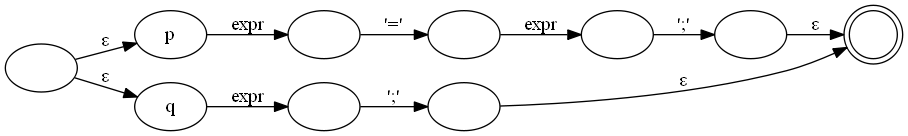
\includegraphics[width=0.9\textwidth]{Figure3.png}
\caption{ATN dla reguły ANTLR stat w gramatyce Ex}
\end{figure}
\par
Ze względu na fakt, iż ALL(*) różni się od deterministycznych zstępujących
metod tylko w mechanizmie przewidywania, możemy utworzyć konwencjonalne parsery
rekurencyjne LL, ale z ważnym wyróżnikiem.
Parsery ALL(*) wywołują specjalne funkcje przewidywania, adaptivePredict,
która analizuje gramatykę w celu utworzenia lookahead DFA
zamiast po prostu porównywać lookahead z statycznie obliczonym zbiorem symboli.
Funkcja adaptivePredict przyjmuje symbole nieterminalne i stos wywołań parsera
jako parametry i zwraca przewidziany numer produkcji lub zgłasza wyjątek,
jeśli nie ma żadnej wykonalnej produkcji. Na przykład, zasada stat z przykładu
w Sekcji 2.1 odzwierciedla analizę składniową przedstawioną na Rysunku 2.
\par
Przewidywanie ALL(*) ma podobną strukturę do znanego algorytmu budowy
podzbiór NFA-to-DFA. Celem jest wykrycie zbioru stanów, które parser może
osiągać po obejrzeniu niektórych lub wszystkich pozostałych danych wejściowych
w stosunku do obecnej decyzji. Podobnie jak w utworzonym podzbiorze,
stan DFA ALL(*) jest możliwym zbiorem konfiguracji analizatora po dopasowaniu
danych wejściowych prowadzących do tego stanu. Zamiast NFA, ALL(*) symuluje
działania rozszerzonej rekurencyjnej sieci przejść (ATN) [27]
odzwierciedlając gramatykę, gdyż ATNs ściśle odzwierciedlają strukturę gramatyki.
\par
(ATNs wyglądają podobnie jak diagramy składniowe, które mogą posiadać działania
i semantyczne predykaty). Statyczna analiza LL(*) również działa w ATN z tego
samego powodu. Rysunek 3 przedstawia podautomat ATN dla zasady stat.
Konfiguracja ATN reprezentuje stan przeprowadzenia subparser i śledzi stan ATN,
przewidziany numer produkcji, oraz stos wywołań subparsera ATN: krotka (p, i, y).
1 Konfiguracje obejmują numery produkcji, tak więc przewidywanie może identyfikować
która produkcja pasuje do bieżącego lookahead.
W przeciwieństwie do analizy statycznej LL(*), ALL(*) stopniowo buduje DFA,
biorąc pod uwagę tylko sekwencje lookahead, zamiast wszystkich możliwych sekwencji.

\begin{figure}[h]
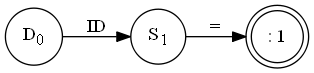
\includegraphics[width=0.32\textwidth]{Figure4a.png}
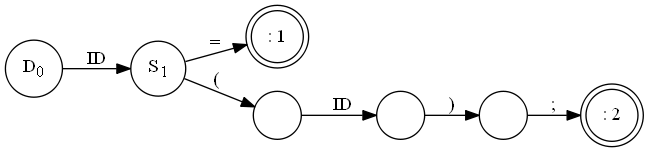
\includegraphics[width=0.64\textwidth]{Figure4b.png}
\\
(po lewo) Po x=y;\\
(po prawo) Po x=y; i f(x);
\caption{Przewidujące DFA dla decyzji stat}
\end{figure}
\par
Gdy analiza składniowa podejmuje decyzję po raz pierwszy, adaptivePredict
inicjuje lookahead DFA dla tej decyzji poprzez utworzenie stanu DFA, $D_0$.
$D_0$ jest zbiorem konfiguracji subparser ATN osiągalnym bez wykorzystywania
początkowego symbolu wejściowego w każdej lewej stronie produkcji.
Na przykład, tworzenie D0 dla nieterminali stat na Rysunku 3 rozpoczyna się
od dodania konfiguracji ATN (p; 1; []) i (q; 2; []) gdzie p i q są stanami
ATN analogicznymi dla produkcji 1 i 2 lewych stron, a [] jest pustym subparserem
stosu wywołań (jeśli stat jest symbolem początkowym).
\par
Analiza następnie oblicza nowy stan DFA, wskazując gdzie symulacja ATN może
być osiągalna po wykorzystaniu pierwszego symbolu lookahead, po czym łączy
dwa stany DFA z krawędzią oznaczoną tym symbolem. Analiza postępuje,
dodając nowe stany DFA, aż wszystkie konfiguracje ATN w nowo utworzonym
stanie DFA przewidują taką samą produkcję: (-; i; -).
Funkcja adaptivePredict uznaje ten stan za akceptowalny i powraca do parsera
z tą liczbą produkcji. Rysunek 4a przedstawia lookahead DFA dla decyzji stat,
po tym jak adaptivePredict przeanalizował zdania wejściowy x = y;.
DFA nie posiada wglądu poza = ponieważ = jest wystarczające, aby jednoznacznie
rozróżnić wyrażenie produkcji. (Zapis: 1 oznacza „przewidywaną produkcję 1”).
\par
Najczęściej adaptivePredict odnajduje istniejący DFA dla konkretnej decyzji.
Celem jest znalezienie lub utworzenie ścieżki poprzez DFA do akceptowalnego stanu.
Jeśli adaptivePredict osiągnie (nieakceptowalny) stan DFA bez krawędzi
dla bieżącego symbolu lookahead, powraca do symulacji ATN aby rozszerzyć DFA
(bez przewijania danych wejściowych). Na przykład, do analizy drugiego zwrotu
danych wejściowych dla stat, takich jak f(x);, adaptivePredict znajduje
istniejącą krawędź ID z D0 i przeskakuje do s1 bez symulacji ATN.
Nie ma żadnego istniejącej krawędzi z s1 dla lewego nawiasu, tak więc analiza
symuluje ATN aby zakończyć ścieżkę do akceptowalnego stanu,
który przewiduje drugą produkcję, zgodnie z Rysunkiem 4b.
Należy zauważyć, że z faktu iż sekwencja ID (ID) przewiduje obie produkcje,
analiza postępuje aż DFA będzie posiadać krawędzie dla symboli = i;.
\par
Jeśli symulacja ATN oblicza nowy stan docelowy, który już istnieje w DFA,
symulacja dodaje nową krawędź nakierowując istniejący stan i przełączając się
na tryb symulacji DFA, począwszy od tego stanu. Nakierowanie istniejących
stanów przedstawia jak cykle mogą pojawiać się w DFA.
Rozszerzając DFA do obsługi nieznanych zwrotów empirycznie zmniejszając
prawdopodobieństwo przyszłych symulacji ATN, tym samym zwiększając szybkość
analizy składniowej (Część 7). 

\subsection{Przewidywania wrażliwe na stos wywołań}
Parsery nie zawsze mogą opierać się na lookahead DFA w podejmowaniu właściwej decyzji.
Aby obsłużyć wszystkie gramatyki nie lewostronnie rekurencyjne,
przewidywanie ALL(*) musi od czasu do czasu rozważyć stos wywołań parsera
dostępnego na początku przewidywania (oznaczone jako 0 w Części 5).
Aby przedstawić potrzebę przewidywań zależnego od stosu, należy wziąć pod uwagę
że przewidywania podczas rozpoznawania metody Javy mogą zależeć od tego
czy metoda została zdefiniowana w ramach definicji klasy lub interfejsu.
(metody interfejsu Java nie mogą posiadać ciała).
Oto przykład uproszczonej gramatyki, która wykazuje decyzję zależną od stosu dla symbolu nieterminalnego A:
\par
\( S \rightarrow xB|yC  \;\;\; B \rightarrow Aa \;\;\; C \rightarrow Aba \;\;\; A \rightarrow b|\varepsilon\)
\\
Bez stosu analizatora, żadna ilość lookahead nie może jednoznacznie rozróżnić
produkcji A. Lookahead ba przewiduje \(A \rightarrow b\) gdy B wywołuje A,
natomiast przewiduje \(A \rightarrow \varepsilon \) gdy C wywołuje A.
W przypadku gdy przewidywanie ignoruje stos wywołań analizatora,
występuje konflikt przewidywania wobec ba.
\par
Parsery, które ignorują stos wywołań analizatora dla przewidywania nazywamy
Silnymi (Strong) LL (SLL). Parsery rekurencyjne programiści tworzą ręcznie
w klasie SLL. Zazwyczaj, literatura odnosi się do SLL jako LL,
ale my rozróżniamy pojęcia, ponieważ „rzeczywiste” LL jest potrzebne aby
obsłużyć wszystkie gramatyki. Powyższa gramatyka to LL(2), a nie SLL(k) dla
jakiegokolwiek k, jednak duplikując A otrzymamy gramatykę SLL (2).
\par
Tworzenie różnych lookahead DFA dla każdego możliwego stosu wywołań
analizatora nie jest możliwe, ponieważ liczba permutacji stosu jest
wykładnicza w funkcji głębokości stosu.
Zamiast tego możemy skorzystać z faktu, iż większość decyzji nie jest zależna
od stosu i utworzyć lookahead DFA ignorując stos wywołań analizatora.
Jeśli symulacja ATN SLL znajduje konflikt przewidywania (Część 5.3),
to nie możemy być pewni czy zwrot lookahead nie jest jednoznaczny
albo zależny od stosu. 
W tym przypadku, adaptivePredict musi ponownie zbadać lookahead używając stosu parsera $\gamma_0$.
Ten hybrydowy lub zoptymalizowany tryb LL zwiększa wydajność poprzez zapisywaniu
w pamięci podręcznej wyników przewidywania niezależnych od stosu w lookahead DFA,
gdy jest to możliwe, przy zachowaniu pełnej siły przewidywania zależnej od siły stosu.
Zoptymalizowany tryb LL stosuje się na podstawie decyzji,
ale dwustopniowa analiza składniowa, opisana w dalszej części,
często może całkowicie uniknąć symulacji LL.
(Od tej pory używamy SLL, aby wskazać analizę składniową niezależną od stosu
i LL do wskazania zależności od stosu).

\subsection{Dwuetapowa analiza składniowa ALL(*)}
SLL jest słabsze, ale szybsze niż LL.
Z faktu iż wykazano, że większość decyzji jest w praktyce SLL, wydaje się
sensowne aby wykonać próbę analizy składniowej wszystkich danych wejściowych
„tylko w trybie SLL”, co jest pierwszym etapem dwuetapowej analizy składniowej algorytmu ALL(*).
Jeśli jednak, tryb SLL wykryje błąd składniowy, wówczas albo jest to słabość SLL
albo prawdziwy błąd składniowy, tak więc musimy ponownie rozpatrzyć wszystkie
dane wejściowe używający zoptymalizowanego trybu LL, który jest drugim etapem.
Ta nieintuicyjna strategia, która potencjalnie parsuje cały strumień wejściowy dwukrotnie,
może dramatycznie zwiększyć prędkość w porównaniu do jednoetapowego zoptymalizowanego trybu LL.
Na przykład, dwu-etapowa analiza składniowa z gramatyką Java (Część 7) jest 8x szybsza
niż jednoetapowy zoptymalizowany tryb LL do przeprowadzania analizy składniowej korpus 123M.
Dwuetapowa strategia opiera się na fakcie, że SLL zachowuje się jak LL
lub otrzymujemy błąd składniowy (Twierdzenie 6.5).
Dla nieprawidłowych zdań, \textbf{nie występuje żadne wyprowadzenie dla danych
wejściowych} niezależnie od tego jak parser wybiera produkcje.
Dla prawidłowych zdań, SLL wybiera produkcje podobnie jak LL albo dobiera produkcję,
która ostatecznie prowadzi do błędu składniowego (LL wykazuje niewykonalny wybór).
Nawet w obecności niejednoznaczności, SLL często rozwiązuje konflikty, podobnie jak LL.
Na przykład, pomimo kilku niejednoznaczności w naszej gramatyce Javy, tryb SLL
poprawnie przeprowadza analizę składniową wszystkich danych wejściowych,
bez doznania niepowodzenia w LL. Niemniej jednak,
drugi etap (LL) musi pozostawać do zapewnienia poprawności.

\section{Gramatyka predykatywna, ATN i DFA}
Aby przeprowadzić formalny proces analizy składniowej ALL(*), najpierw należy przypomnieć sobie niektóre materiały, zwłaszcza formalne definicje gramatyki predykatowej, ATN i Lookahead DFA.

\subsection{Gramatyka predykatowa}
Aby przeprowadzić formalny proces analizy składniowej ALL(*), najpierw należy formalnie
określić gramatykę predykatową z której jest ona czerpana.
Gramatyka predykatowa \(G = (N, T, P, S, \Pi, \mathcal{M})\) składa się z następujących elementów: 
\begin{itemize}
\item N jest zbiorem nie-terminali (nazwy reguł) 
\item T jest zbiorem terminali (symboli) 
\item P jest zbiorem produkcji 
\item \(S \in N\) jest symbolem początkowym 
\item \( \Pi \) jest zbiorem efektów ubocznych semantycznych predykatów
\item \(\mathcal{M}\) jest zbiorem działań (mutatorów) 
\end{itemize}
Gramatyki predykatowe ALL(*) różnią się od tych z LL(*) [20] jedynie tym że
gramatyka ALL(*) nie potrzebuje albo nie obsługuje składni predykatów.
Gramatyki predykatowe w formalnych częściach niniejszego dokumentu używają
notacji przedstawionej na Rysunku 5.
Zasady wyprowadzania na Rysunku 6 określają znaczenie gramatyki predykatowej.
Do obsługi semantycznych predykatów i mutatorów, zasady odnoszą się do stanu S,
który abstrahuje stan użytkownika podczas analizowania.
Przejście \(( \mathbb{S}, \alpha) \Rightarrow ( \mathbb{S'}, \beta) \)
może zostać odczytane: „W stanie S maszyny, sekwencja gramatyczna \(\alpha\)
redukuje się w jednym kroku do zmodyfikowanego stanu S' i sekwencji gramatycznej \(\beta\)”.
Przejście \((\mathbb{S}, \alpha) \Rightarrow^* (\mathbb{S'}, \beta)\)
oznacza wielokrotne zastosowanie jednostopniowej zasady redukcji.
Te zasady redukcji określają wyprowadzenie lewostronne.
Produkcja z semantycznym predykatem \(\pi_i\) jest wykonalna tylko wtedy,
gdy \(\pi_i\) jest true z bieżącym stanem \(\mathbb{S}\).
Na koniec akcja produkcji używa określonego mutatora \(\mu_i\) aby zaktualizować stan.
\par
Formalnie, język generowany przez sekwencję gramatyczną \(\alpha\)
w stanie użytkownika \(\mathbb{S}\)
jest \(L(\mathbb{S},\alpha) = \{w| (\mathbb{S},\alpha)\Rightarrow^*(\mathbb{S'},w)\} \)
a język gramatyki G jest \(L(\mathbb{S}_0,G) = \{w| (\mathbb{S}_0,S)\Rightarrow^*(\mathbb{S},w)\} \)
dla początkowego stanu \(\mathbb{S}_0\) użytkownika (\(\mathbb{S}_0\) może być puste).
Jeśli \(\mu\) jest przedrostkiem \(w\) albo równe \(w\), zapisujemy \(\mu \preceq w\).
Język L jest ALL(*) wtedy i tylko wtedy jeśli występuje gramatyka ALL(*) dla L.
Teoretycznie, klasa języka L(G) jest rekurencyjnie przeliczalna,
ponieważ każdy mutator może być maszyną Turinga.
W rzeczywistości, autorzy gramatyki nie wykorzystują tego ogólnika,
tak więc jest to przyjęty sposób postępowania do rozważenia klasy języka,
zamiast kontekstowego języka. Klasa jest zależna od kontekstu, a nie bezkontekstowa,
ponieważ predykaty mogą badać stos wywołań i terminale z lewej i prawej.
\par
Ten formalizm uwzględnia różne składniowe ograniczenia, które nie są obecne w rzeczywistej
gramatyce ANTLR, na przykład zmuszając mutatory do ich własnych zasad i wykluczając
powszechne notacje Rozszerzonego (Extended) BNF (EBNF),
takie jak domknięcia \(\alpha^*\) i \(\alpha^+\).
Możemy ustalić te ograniczenia bez utraty ogólnika, ponieważ jakakolwiek
gramatyka w ogólnej formie może przekładać się na bardziej ograniczoną formę. 

\subsection{Sprecyzowanie niejednoznaczności}
Niejednoznaczna gramatyka jest taką, w który taka sama sekwencja danych wejściowych
może być rozpoznawana na wiele sposobów.
Zasady na Rysunku 6 nie wykluczają niejednoznaczności. 

\begin{figure}[h]
\noindent\rule{\linewidth}{1pt} \\
\( A \in N \) symbol nieterminalny \\
\( a,b,c,d \in T \) symbol terminalny \\
\( X \in (N \cup T) \) element produkcji \\
\( \alpha,\beta,\delta \in X^* \) sekwencja symboli gramatyki \\
\( u,v,w,x,y \in T^* \) sekwencja symboli terminalnych \\
\( \varepsilon \) pusty ciąg \\
\$ koniec strumienia symboli \\
\( \pi \in \Pi \) predykat w języku docelowym \\
\( \mu \in \mathcal{M} \) akcja w języku docelowym \\
\( \lambda \in (N \cup \Pi \cup \mathcal{M}) \) etykieta redukcji \\
\( \overset{\rightarrow}{\lambda} = \lambda_1 ..\lambda_n\) sekwencja etykiet redukcji \\
Reguły produkcji:\\
\( A \rightarrow \alpha_i \) i-ta bezkontekstowa produkcja A \\
\( A \rightarrow \{ \pi_i \} ? \alpha_i \) i-ta produkcja predykowana na semantyce \\
\( A \rightarrow \{ \mu_i \} \) i-ta produkcja z mutatorem \\
\noindent\rule{\linewidth}{1pt} 
\caption{Notacja gramatyki predykatowej}
\end{figure}

\begin{figure}[h]
\noindent\rule{\linewidth}{1pt} \\
\begin{adjustwidth}{2cm}{}
Prod \( \frac{A \rightarrow \alpha}{ (\mathbb{S}, uA\delta) \Rightarrow (\mathbb{S}, u\alpha\delta)} \) 
\\
\( \pi(\mathbb{S}) \)
\\
Sem \( \frac{A \rightarrow \{ \pi \} ? \alpha}{ (\mathbb{S}, uA\delta) \Rightarrow (\mathbb{S}, u\alpha\delta)} \) 
\\
Action \( \frac{A \rightarrow \{ \mu \} }{ (\mathbb{S}, uA\delta) \Rightarrow (\mu (\mathbb{S}), u\delta)} \) 
\\
Closure \( \frac{ (\mathbb{S},\alpha) \Rightarrow (\mathbb{S'},\alpha'),
(\mathbb{S'},\alpha') \Rightarrow^* (\mathbb{S''},\beta) }{(\mathbb{S},\alpha) \Rightarrow^* (\mathbb{S''},\beta)} \) 
\\
\end{adjustwidth}
\noindent\rule{\linewidth}{1pt}
\caption{Reguły lewostronnego wyprowadzania gramatyki predykatowej}
\end{figure}

Jednakże, dla praktycznego analizatora języka programowania,
wszystkie dane wejściowe powinny odpowiadać analizie składniowej.
W tym celu, ALL(*) używa kolejności produkcyjnych w regule do rozpoznania
niejednoznaczności na korzyść produkcji o najniższym numerze.
Strategia ta jest zwięzłym sposobem dla programistów, aby rozpoznać niejednoznaczności
automatycznie oraz znaną niejednoznaczność if-then-else w zwykły sposób
poprzez kojarzenie ‘else’ z ostatnim ‘if’. Parsery PEG i Bison mają te same zasady rozpoznawania.
\par
Do rozpoznania niejednoznaczności, które zależą od bieżącego stanu S, programiści mogą
wprowadzać semantyczne predykaty, jednakże muszą wzajemnie wykluczyć dla wszystkich
potencjalnie niejednoznacznych sekwencji wejściowych do otrzymania tego typu jednoznacznych produkcji.
Statycznie wzajemnych wykluczeń nie da się wymusić, ponieważ predykaty są napisane w języku Turinga.
Jednakże, w czasie analizy ALL(*) wylicza predykaty i dynamicznie raportuje
frazy wejściowe dla których wielokrotne, predykowalne produkcje są wykonalne.
Jeśli programistom nie udaje się ustalić wzajemnej wyłączności, ALL(*)
wykorzystuje kolejność produkcji do rozpoznania niejednoznaczności.

\subsection{Rozszerzone sieci przejść}
Biorąc pod uwagę gramatykę predykatową \(G = (N, T, P, S, \Pi, \mathcal{M})\)
odpowiedni ATN \(M_G = (Q, \Sigma, \Delta, E, F) \) ma elementy [20]: 
\begin{itemize}
\item Q jest zbiorem stanów
\item \( \Sigma \) jest alfabetem krawędzi \( N \cup T \cup  \Pi \cup \mathcal{M}\)
\item \( \Delta \) relacją przejść mapującą \( Q \times (\Sigma \cup \epsilon) \rightarrow Q \) 
\item \( E \subset Q = \{p_A|A \in N\} \) jest zbiorem stanów początkowych subautomatu
\item \( F \subset Q = \{p'_A|A \in N\} \) jest zbiorem stanów końcowych subautomatu
\end{itemize}

\begin{figure}[h]
\begin{tabular}{c|c} 
  \hline
  \head{Element gramatyki wejściowej} & \head{Wynikowe przejścia ATN} \\
  \hline
  \(A \rightarrow \alpha_i \) & \(p_A \overset{\epsilon}{\rightarrow} p_{A,i}
                  \overset{\epsilon}{\rightarrow} \boxed{\alpha_i} \overset{\epsilon}{\rightarrow} p'_A \) \\
  \(A \rightarrow \{ \pi_i \}? \alpha_i \) & \(p_A \overset{\epsilon}{\rightarrow} p_{A,i}
                  \overset{\pi_i}{\rightarrow} \boxed{\alpha_i} \overset{\epsilon}{\rightarrow} p'_A \) \\
  \(A \rightarrow \{ \mu_i \}  \) & \(p_A \overset{\epsilon}{\rightarrow} p_{A,i}
                  \overset{\mu_i}{\rightarrow} p'_A \) \\
  \(A \rightarrow  \epsilon_i \) & \(p_A \overset{\epsilon}{\rightarrow} p_{A,i}
                  \overset{\epsilon}{\rightarrow} p'_A \) \\
  \( \boxed{\alpha_i} = X_1X_2...X_m \) \\ for \( X_j \in N \cup T \),j=1..m  & \( p_0
                  \overset{X_1}{\rightarrow} p_1 \overset{X_2}{\rightarrow} ... \overset{X_m}{\rightarrow} p_m \) \\
  \hline
\end{tabular}
\caption{Transformacja gramatyki predykatowej do ATN}
\end{figure}

\begin{figure}[h]
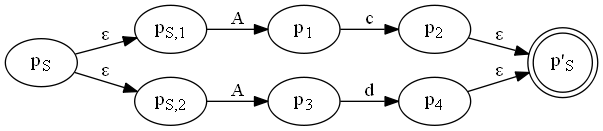
\includegraphics[width=0.45\textwidth]{Figure8a.png}
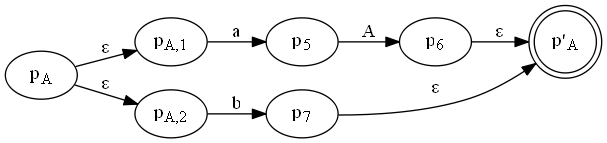
\includegraphics[width=0.45\textwidth]{Figure8b.png}
\caption{ATN dla G z \( P = \{S \rightarrow Ac|Ad, A \rightarrow aA|b \} \)}
\end{figure}

ATNy przypominają diagramy składni, używane do dokumentowania języków programowania,
z podautomatami ATN dla poszczególnych symboli nieterminalnych.
Rysunek 7 przedstawia jak utworzyć zbiór stanów Q i krawędzie \( \Delta \)
z produkcji gramatyki. Początkowy stan dla A jest \( p_A \in Q \)
i jest skierowany na \( p_{A,i} \) utworzony z lewej strony krawędzi \( \alpha_i \) ,
z krawędzią w \( \Delta \). Ostatni stan utworzony z \( \alpha_i \) jest skierowany na \( p'_A \).
Nieterminalne krawędzie \( p \overset{A}{\rightarrow} q\) są niczym wywołania funkcji.
Przenoszą kontrolę ATN na podautomat A, wkładając stan powrotny q na stos wywołań,
tak aby mógł kontynuować z q po osiągnięciu stanu stop dla A podautomatu \( p'_A \).
Rysunek 8 przedstawia ATN dla prostej gramatyki.
Język rozpoznawany przez ATN jest taki sam, jak oryginalny język gramatyczny.

\subsection{Lookahead DFA}
Parsery ALL(*) odnotowują wyniki przewidywań uzyskane z symulacji ATN wraz z lookahead DFA,
które są rozszerzonym DFA z akceptowalnymi stanami, odzwierciedlającymi numer przewidywanej produkcji.
Występuje jeden akceptowalny stan decyzji na produkcję.
Definicja 4.1. Lookahead DFA to DFA rozszerzony o akceptujące stany,
który dostarcza numer przewidywanej produkcji.
Dla gramatyki predykatowej \(G = (N, T, P, S, \Pi, \mathcal{M}), DFA M = (Q, \Sigma, \Delta, D_0, F) \) gdzie
\begin{itemize}
\item Q jest zbiorem stanów
\item \(\Sigma = T \)jest alfabetem krawędzi
\item \( \Delta \) jest funkcją przejścia mapującą \( Q \times \Sigma \rightarrow Q \)
\item \( D_0 \in Q \) jest stanem startowym
\item \( F \subset Q  = \{  f_1, f_2, ..., f_n\}\) stany końcowe, jeden \( f_i \)  dla produkcji i
\end{itemize}
Przejście w \( \Delta \) ze stanu p do stanu q na symbolu \( a \in \Sigma \)
ma postać \( p \overset{a}{\rightarrow} q \) i wymagamy by \(p \overset{a}{\rightarrow} q' \)
implikowało  q = q'.


\section{Algorytm analizy składniowej ALL(*)}
Z definicji gramatyki, sformalizowanych ATN i lookahead DFA, możemy przedstawić główne funkcje
algorytmu analizy składniowej ALL(*).
W części tej podsumowujemy wszystkie funkcje i opisujemy jak łączą się one, następnie omawiamy
krytyczną strukturę danych przed przedstawianiem samych funkcji. Ostatecznie przedstawimy
przykład jak działa algorytm.
\par
Parsowanie rozpoczyna się od funkcji \textit{parse}, która zachowuje się jak konwencjonalna
zstępująca analiza funkcji LL(k), z wyjątkiem tego że parsery ALL(*) przewidują
produkcje ze specjalną funkcją zwaną \textit{adaptivePredict},
zamiast zwykłego mechanizmu „przełącz na następny typ symbolu k”.
Funkcja \textit{adaptivePredict} symuluje ATN odzwierciedlając pierwotną gramatykę
predykatu w wyborze produkcji $\alpha_i$ w celu rozwinięcia punktu decyzyjnego
$A \rightarrow \alpha_1 | ... | \alpha_n$.
Od strony koncepcyjnej, przewidywanie jest funkcją bieżącej analizy składniowej stosu wywołań
$\gamma_0$, pozostałych danych wejściowych $w_r$ i stanu użytkownika $\mathbb{S}$ jeśli A posiada predykaty.
Jeżeli chodzi o wydajność, przewidywanie ignoruje $\gamma_0$, gdy to tylko możliwe (Sekcja 3.1)
i używa minimalnego lookahead z $w_r$.
\par
Aby uniknąć powtarzania symulacji ATN dla tych samych danych wejściowych i symboli nieterminalnych,
\textit{adaptivePredict} składa DFA, który gromadzi mapowania danych wejściowych do przewidywanej produkcji,
jeden DFA na symbol nieterminalny.
Należy mieć na uwadze, że każdy stan DFA, D, jest zbiorem konfiguracji ATN dopuszczalnym po dopasowaniu
symboli lookahead prowadzących do tego stanu.
Funkcja \textit{adaptivePredict} wywołuje \textit{startState} do utworzenia początkowego stanu DFA,
\( D_0 \) a następnie wywołuje \textit{SLLpredict} w celu uruchomienia symulacji.
\par
Funkcja \textit{SLLpredict} dodaje ścieżki do lookahead DFA, które pasują do niektórych lub wszystkich
$w_r$ poprzez wielokrotne wołanie \textit{target}. Funkcja \textit{target} oblicza DFA docelowego stanu D'
z bieżącego stanu D przy użyciu operacji \textit{move} i \textit{closure} podobnych do tych
znalezionych w \textit{subset construction}.
Funkcja \textit{move} wykrywa wszystkie konfiguracje ATN jako osiągalne na bieżącym symbolu wejściowym,
a funkcja \textit{closure} wykrywa wszystkie konfiguracje jako osiągalne bez przemierzenia krawędzi terminalnej.
Podstawową różnicą od podzbioru konstrukcji jest to, że \textit{closure} symuluje wywołanie
i powrót podautomatów ATN związanych z symbolami nieterminali.
\par
W przypadku, gdy symulacja SLL wykryje konflikt (Sekcja 5.3), \textit{SLLpredict} odwija dane wejściowe
i wywołuje \textit{LLpredict} w celu ponowienia próby przewidywania, tym razem biorąc pod uwagę $\gamma_0$.
Funkcja \textit{LLpredict} jest podobna do \textit{SLLpredict}, ale nie aktualizuje symboli nieterminalnych
DFA, ponieważ DFA musi być niezależny od stosu, aby mógł być wykorzystywany we wszystkich kontekstach stosu.
Konflikty w zbiorach konfiguracji ATN wykryte przez \textit{LLpredict} reprezentują niejednoznaczności.
Obie funkcje przewidywania używają \textit{getConflictSetsPerLoc} do wykrywania konfliktów,
które są konfiguracjami określającymi tą samą lokalizację parsera, ale różne produkcje.
Aby uniknąć niepowodzenia \textit{LLpredict}, \textit{SLLpredict} wykorzystuje \textit{getProdSetsPerState}
aby zobaczyć czy potencjalnie bezkonfliktowa ścieżka DFA pozostaje gdy \textit{getConflictSetsPerLoc}
zgłasza konflikt.
Jeśli tak, to warto kontynuować proces \textit{SLLpredict}, mając nadzieję że więcej lookahead
rozwiąże konflikt bez uciekania się do pełnej analizy składniowej LL.
\par
Zanim szczegółowo omówimy te funkcje, przedstawimy przegląd fundamentalnych danych struktury grafu,
które efektywnie zarządzają wieloma stosami wywołań GLL i GLR.

\subsection{Stosy wywołań o strukturze grafowej}
Najprostszym sposobem implementacji przewidywania ALL(*) byłoby klasyczne podejście
algorytmu z nawrotami (backtrackingu), uruchamiając subparser dla każdego $\alpha_i$.
Subparsery przetworzą wtedy wszystkie pozostałe dane wejściowe, ponieważ algorytm z nawrotami
subparserów nie wie kiedy zaprzestać analizy – nie zna statusu pozostałych subparserów.
Niezależne subparsery wywołałyby również gwałtowną złożoność czasową.
Zajęliśmy się obiema kwestiami poprzez postępowanie przewidujących subparserów równym krokiem
poprzez $w_r$. Przewidywanie wygasa po przetworzeniu przedrostka $u \preceq w_r$,
gdy wszystkie subparsery oprócz jednego zamierają lub przewidywanie identyfikuje konflikt.
Praca w równym kroku również stanowi okazję dla subparserów do podziału stosów wywołań,
w ten sposób unikając zbędnych obliczeń.
\par
Dwa subparsery w stanie ATN-u p, które dzielą taki sam szczyt stosu ATN,
$q\gamma_1$ i $q\gamma_2$, odzwierciedlają takie samo zachowanie dotąd aż symulacja pobierze q ze stosów.
Przewidywanie może traktować te subparsery jako pojedynczy subparser poprzez łączenie stosów.
Możemy łączyć stosy dla wszystkich konfiguracji w stanie DFA w postaci $(p,i,\gamma_1)$ oraz $(p,i,\gamma_2)$,
tworząc ogólną konfigurację $(p,i,\Gamma)$ z \textit{graph-structured stack} (GSS) [25]
$\Gamma = \gamma_1 \uplus \gamma_2$ gdzie $\uplus$ określa połączenie.
$\Gamma$ może być pustym stosem [], specjalnym stosem \# wykorzystywanym do przewidywania SLL (wkrótce się odniesiemy),
indywidualnym stosem, albo grafem węzłów stosu.
Łączenie poszczególnych stosów w GSS zmniejsza potencjalną wielkość wykładniczej do złożoności liniowej
(Twierdzenie 6.4). Do reprezentacji GSS używamy niezmiennej struktury danych grafu
z maksymalnym współdzieleniem węzłów.
Oto dwa przykłady, które dzielą stos parsera $\gamma_0$ w dolnej części stosu:
\par
\parbox{\columnwidth}{
  \parbox{0.8in}{
    \centering
    $p \gamma_0 \uplus q \gamma_0 =$
  }
  \parbox{0.5in}{
    \centering
    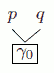
\includegraphics[scale=0.5]{5_1a}
  }
  \parbox{1.3in}{
    \centering
    $q \Gamma \gamma_0 \uplus q \Gamma' \gamma_0 =$
  }
  \parbox{0.5in}{
    \centering
    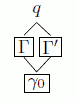
\includegraphics[scale=0.5]{5_1b}
  }
}
\par
W funkcjach, które omówimy, wszystkie dodatki do zbiorów konfiguracji, takie jak w przypadku operatora +=, domyślnie łączą stosy.
\par
Występuje szczególny przypadek związany z warunkiem stosu na początku przewidywania.
$\Gamma$ musi rozróżniać pomiędzy pustym stosem a brakiem informacjami stosu.
Dla przewidywania LL, początkowa symulacja stosu ATN jest bieżącym parserem stosu wywołań $\gamma_0$.
Początkowy stos jest pusty, $\gamma_0$ = [], gdy reguła decyzji wejścia jest symbolem startowym.
Przewidywanie SLL niezależne od stosu, z drugiej strony, ignoruje parser stosu wywołań i używa początkowego
stosu \# wskazując brak informacji stosu.
To rozróżnienie jest ważne obliczając \textit{closure} (Funkcja 7) konfiguracji
stanowiące stan zatrzymania podmaszyny. Bez informacji stosu parsera, subparser który zwraca
z decyzji wejścia regułę A musi wziąć pod uwagę wszystkie możliwe wywołania miejsc
czyli \textit{closure} widzi konfigurację ($p'_A$,-,\#).
\par
Pusty stos [] jest traktowany podobnie jak inne węzły do przewidywania LL:
$\Gamma \uplus []$ przedstawia grafową równowartość zbioru $\{\Gamma, []\}$,
co oznacza że zarówno $\Gamma$ jak i pusty stos są dopuszczalne.
Wkładając stan p na [] mamy p[], a nie p, ponieważ pobranie p musi pozostawić symbol pustego stosu.
Dla przewidywania SLL, $\Gamma \uplus \# = \#$ dla dowolnego grafu $\Gamma$, ponieważ \# stanowi symbol
wieloznaczny i reprezentuje zbiór wszystkich stosów. Dlatego też, znak wieloznaczny zawiera wszelkie
$\Gamma$. Wkładając stan p na \# mamy p\#.


\subsection{Funkcje parsowania ALL(*)}
Teraz możemy omówić kluczowe funkcje ALL(*), które zostały zaznaczone w boksach
i wymienione poniżej. Niniejszy opis został zapisany w zstępującym porządku i zakłada
że ATN odpowiadający gramatyce G, semantyczny stan $\mathbb{S}$, tworzone DFA, oraz dane wejściowe
są odpowiednie dla wszystkich funkcji algorytmu i że semantyczne predykaty oraz działania
mogą mieć bezpośredni dostęp do $\mathbb{S}$.
\par
\textbf{Funkcja parse}. Głównym punktem wejściowym jest funkcja \textit{parse}
(przedstawiona w Funkcji 1), która inicjuje parsowanie z początkowym symbolem, argument S.
Funkcja rozpoczyna się od uruchomienia symulacji stosu wywołań $\gamma$ do pustego stosu
i ustawienia „kursora” stanu ATN $p$ na $p_{S,i}$ stanu ATN w lewej krawędzi produkcji S
o numerze i przewidzianego za pomocą \textit{adaptivePredict}.
Funkcja jest w pętli do czasu gdy kursor osiągnie stan zatrzymania $p'_S$ podmaszyny dla S.
Gdy kursor osiągnie kolejny stan zatrzymania podmaszyny $p'_B$, funkcja \textit{parse}
symuluje „powrót” wyświetlając stan powrotny q ze stosu wywołań i przenosząc p do q.
\\
\minibox[frame]{\textbf{Function 1}:parse(S)\\
$\gamma$ := []; i:=adaptivePredict(S,$\gamma$); p:=$p_{S,i}$; \\
\textbf{while} true \textbf{do} \\
\tab \textbf{if} p=$p'_B$ \{czyli p jest regułą stanu stop\} \textbf{then} \\
\tab \tab \textbf{if} B=S \{startowa reguła S końcowego dopasowania\} \textbf{then return}; \\
\tab \tab \textbf{else let} $\gamma=q\gamma'$ \textbf{in} $\gamma:=\gamma'$; p:=q; \\
\tab \textbf{else} \\
\tab \tab \textbf{switch} t where $p \overset{t}{\rightarrow} q$ \textbf{do} \\
\tab \tab \tab \textbf{case} b: \{ czyli przejście symbolu terminalnego\} \\
\tab \tab \tab \tab \textbf{if} b=input.curr() \textbf{then}\\
\tab \tab \tab \tab \tab p:=q; input.advance();\\
\tab \tab \tab \tab \textbf{else} parse error;\\
\tab \tab \tab \textbf{case} B: $\gamma:=q\gamma$;i:=adaptivePredict(B,$\gamma$); p:=$p_{B,i}$; \\
\tab \tab \tab \textbf{case} $\mu$: $\mathbb{S}$:=$\mu(\mathbb{S})$; p:=q; \\
\tab \tab \tab \textbf{case} $\pi$: \textbf{if} $\pi(\mathbb{S})$ \textbf{then} p:=q \textbf{else} parse error; \\
\tab \tab \tab \textbf{case} $\epsilon$: p:=q; \\
\tab \tab \textbf{endsw} \\
}
\par
Dla p nie w stanie zatrzymania, analiza dokonuje przejścia ATN $p\overset{t}{\rightarrow}q$.
Może wystąpić tylko jedno przejście z p, ze względu na sposób w jaki ATNy są utworzone.
Jeśli t jest symbolem terminalnym krawędzi i pasuje do bieżącego symbolu wejściowego,
\textit{parse} przechodzi przez krawędź i przechodzi do następnego symbolu.
Jeśli t jest symbolem nieterminalnym krawędzi, odwołującym się do niektórych B, \textit{parse} symuluje
wywołania podmaszyny wkładając stan powrotny q na stos i wybierając odpowiednie produkcje lewej krawędzi w B
poprzez wywołanie \textit{adaptivePredict} i ustawiając odpowiednio kursor.
Dla krawędzi akcji, \textit{parse} aktualizuje stan zgodnie z mutatorem i przechodzi do q.
Dla krawędzi predykatu, parse przechodzi tylko jeśli predykat $\pi$ ocenia za prawdziwy.
Podczas parsowania, niezatwierdzone predykaty zachowują się jak niedopasowane symbole.
Dla krawędzi $\epsilon$, \textit{parse} przechodzi do q.
Funkcja \textit{parse} nie sprawdza jawnie czy parsowanie zatrzymuje się na końcu pliku,
ponieważ aplikacje, takie jak środowisko programistyczne powinny parsować wejściowe podfrazy.
\par
\textbf{Funkcja adaptivePredict}. Do przewidywania produkcji, \textit{parse} wywołuje \textit{adaptivePredict}
(Funkcja 2), która jest funkcją decyzji symboli nieterminalnych A i bieżącego stosu analizatora $\gamma_0$.
Ponieważ w trakcie pełnej symulacji LL przewidywanie ocenia tylko predykaty, \textit{adaptivePredict}
przechodzi do \textit{LLpredict} jeśli przynajmniej jedna z produkcji jest predykatem.\footnotemark[5]
\footnotetext[5]{
Predykcja SLL nie włącza predykatów dla czytelności w tym naświetleniu tematu,
ale w praktyce ANTLR włącza predykaty do stanów akceptowalnych DFA (Sekcja B.2).
DFA ANTLR 3 używało predykatowych krawędzi a nie predykatowych stanów akceptujących.}
W przypadku decyzji, które nie posiadają jeszcze DFA, \textit{adaptivePredict} tworzy DFA $dfa_A$
z początkowym stanem $D_0$ w przygotowaniu do \textit{SLLpredict} aby dodać ścieżki DFA.
$D_0$ jest zbiorem konfiguracji ATN osiągalnym bez przechodzenia przez krawędzie terminali.
Funkcja \textit{adaptivePredict} tworzy również zbiór stanów końcowych $F_{DFA}$,
który zawiera jeden stan końcowy $f_i$ dla każdej produkcji A. Zbiór stanów DFA, $Q_{DFA}$,
jest powiązany z $D_0$, $F_{DFA}$ oraz stanem błędu $D_{error}$.
Słownik $\Sigma_{DFA}$ to zbiór terminali gramatycznych T.
W przypadku nieprzewidzianych decyzji z istniejącym DFA, \textit{adaptivePredict} wywołuje
\textit{SLLpredict} do uzyskania przewidywania z DFA, z możliwością rozszerzenia DFA poprzez
symulację ATN w procesie.
Ostatecznie, z faktu iż \textit{adaptivePredict} tylko przegląda, a nie przeprowadza analizy składniowej,
musi cofnąć jakiekolwiek zmiany wprowadzone do kursora wejściowego,
poprzez przechwytywanie indeksu wejściowego jako start na początku przewijanie na początek przed wyjściem.
\\
\minibox[frame]{\textbf{Function 2}:adaptivePredict(A,$\gamma_0$) \textbf{returns} int alt\\
start:=input.index(); // checkpoint input \\
\textbf{if} $\exists A \rightarrow \pi_i \alpha_i $ \textbf{then} \\
\tab alt:=LLpredict(A,start,$\gamma_0$); \\
\tab input.seek(start); //wycofanie zmian pozycji strumienia \\
\tab return alt; \\
\textbf{if} $\nexists dfa_A$ \textbf{then} \\
\tab $D_0$ := startState(A,\#);\\
\tab $F_{DFA}$ := \{ f_i | f_i:=DFA.State(i) $\forall A \rightarrow \alpha_i $\} \\
\tab $Q_{DFA}$ := $D_0 \cup F_{DFA} \cup  D_{error} $ \\
\tab $dfa_A$ := DFA($Q_{DFA},\Sigma_{DFA}=T,\Delta_{DFA}=\varnothing, D_0,F_{DFA}$); \\
alt:=SLLpredict(A,$D_0$,start,$\gamma_0$); \\
input.seek(start);  //wycofanie zmian pozycji strumienia \\
return alt;
} \\
\par
\textbf{Funkcja startState}. Aby utworzyć startowy stan DFA $D_0$,
\textit{startState} (Funkcja 3) dodaje konfiguracje $(p_{A,i}, i, \gamma)$
dla każdego $A \rightarrow \alpha_i$ oraz $A \rightarrow \pi_i \alpha_i$,
jeśli $\pi_i$ oceniony jako prawdziwy.
W przypadku wywołania z \textit{adaptivePredict} argument stosu wywołań $\gamma$
jest specjalnym symbolem \# wymaganym przez predykcję SLL, wskazując „brak informacji stosu analizatora”.
W przypadku wywołania z \textit{LLpredict}, $\gamma$ jest początkowym stanem stosu
analizatora $\gamma_0$.
Obliczenie \textit{closure} konfiguracji skompletuje $D_0$.
\\
\minibox[frame]{\textbf{Function 3}:startState(A,$\gamma$) \textbf{returns} DFA.State $D_0$\\
$D_0:=\varnothing$ \\
\textbf{foreach} $p_A \overset{\epsilon}{\rightarrow} p_{A,i} \in \Delta_{ATN}$ \textbf{do}\\
\tab \textbf{if} $p_A \overset{\epsilon}{\rightarrow} p_{A,i}\overset{\pi_i}{\rightarrow} p $
     \textbf{then} $\pi:=\pi_i $ \textbf{else} $\pi:=\epsilon $; \\
\tab \textbf{if} $\pi=\epsilon $ or eval($\pi_i $) \textbf{then} $D_0$ += closure(\{\}, $D_0,(p_{A,i},i,\gamma) $);\\
return $D_0$;
} \\
\par
\textbf{Funkcja SLLpredict}. Funkcja \textit{SLLpredict} (Funkcja 4) dokonuje zarówno symulację
DFA jak i SLL ATN, stopniowo dodając ścieżki do DFA.
W najlepszym przypadku, występuje już ścieżka DFA z $D_0$ do akceptowalnego stanu, $f_i$
dla przedrostka $u \preceq w_r$ i pewnej produkcji o numerze $i$.
W najgorszym przypadku symulacja ATN jest wymagana dla wszystkich $a$ w sekwencji $u$.
Główna pętla w \textit{SLLpredict} znajduje istniejącą krawędź wychodzącą ze stanu DFA
kursora D w $a$ lub oblicza nową za pomocą \textit{target}.
Możliwe jest że \textit{target} obliczy stan docelowy \underline{D'}, który już istnieje w DFA,
w którym funkcja \textit{target} zwraca \underline{D'};
ponieważ \underline{D'} może już mieć obliczone krawędzie wychodzące,
nieefektywne jest odrzucenie pracy przez zastępując \underline{D'}.
W następnej iteracji, SLLpredict rozważy krawędzie z \underline{D'},
skutecznie przełączając na symulację DFA.
\\
\minibox[frame]{\textbf{Function 4}:SLLpredict(A,$D_0, start, \gamma_0$) \textbf{returns} int prod\\
a:=input.curr(); D = $D_0$;\\
\textbf{while} true \textbf{do}\\
\tab \textbf{let} D' be DFA target $D \overset{a}{\rightarrow}D'$ \\
\tab \textbf{if} D'=$D_{error}$ then parse error; \\
\tab \textbf{if} D' stack sensitive \textbf{then}\\
\tab \tab input.seek(start); return LLredict(A,start, $\gamma_0$); \\
\tab \textbf{if} D'=$f_i \in F_{DFA}$ \textbf{then return} i;\\
\tab D:=D'; a:=input.next();
}
\par
Gdy tylko \textit{SLLpredict} osiągnie stan docelowy D', wówczas sprawdza
pod kątem błędów, zależności stosu i ukończenia.
W przypadku gdy \textit{target} D' jest oznaczony jako zależny od stosu,
przewidywanie wymaga pełnej symulacji LL, a \textit{SLLpredict} wywołuje \textit{LLpredict}.
W przypadku gdy D' jest akceptowalnym stanem $f_i$ jsko określone przez \textit{target},
\textit{SLLpredict} zwraca $i$.
W tym przypadku, wszystkie konfiguracje w D' przewidują taką samą produkcję i.
Dalsza analiza nie jest już potrzebna, a algorytm może zostać zatrzymany.
Dla jakiegokolwiek innego D' algorytm ustawia D na D', pobiera następny symbol i powtarza.
\par
\textbf{Funkcja target}. Przy użyciu połączonych operacji \textit{move-closure}
funkcja \textit{target} wykrywa zbiór konfiguracji ATN osiągalny z D
na jednym symbolu terminalnym $a \in T$. Funkcja \textit{move} oblicza konfiguracje
osiągalne bezpośrednio na a poprzez przejście terminalnej krawędzi:
\par
move(D,a) = \{$(q,i,\Gamma) | p \overset{a}{\rightarrow} q, (p,i,\Gamma)\in D $\}
\par
Te konfiguracje i ich \textit{closure} formują D'.
Jeśli D' jest puste, żadna alternatywa nie jest wykonalna, ponieważ żadna nie może dopasować
$a$ z bieżącego stanu, tak więc \textit{target} zwraca stan błędu $D_{error}$.
Jeśli wszystkie konfiguracje w D' przewidują taki sam numer produkcji i,
\textit{target} dodaje krawędź $D \overset{a}{\rightarrow} f_i$ i zwraca stan akceptowalny $f_i$.
Jeśli D' ma konfliktujące konfiguracje, \textit{target} zaznacza D' jako zależny od stosu.
Konfliktem może być niejednoznaczność albo słabość wynikająca z braku informacji stosu parsera SLL.
(Konflikty wraz z \textit{getConflictSetsPerLoc} i \textit{getProdSetsPerState} zostały opisane w Sekcji 5.3).
Funkcja kończy poprzez dodanie stanu D', jeśli odpowiedni stan \underline{D'} nie występuje już w DFA,
oraz dodając krawędź $D\overset{a}{\rightarrow}D'$.
\\
\minibox[frame]{\textbf{Function 5}:target(D,a) \textbf{returns} DFA.State D'\\
mv:=move(D,a);\\
D':=$\bigcup_{c \in mv}^{}$ closure(\{\},c);\\
\textbf{if} D'=$\varnothing$ \textbf{then} $\Delta_{DFA}$ += $D\overset{a}{\rightarrow}D_{error}$;
            \textbf{return} $D_{error}$; \\
\textbf{if} \{ j|(-,k,-)$\in D'$\} = \{i\} \textbf{then} \\
\tab $\Delta_{DFA}+=D\overset{a}{\rightarrow}f_i$; \textbf{return} $f_i$;//Predykcja reguły i \\
//Patrz na konflikt między konfiguracjami D' \\
a.conflict:=$\exists alts \in$getConflictSetsPerLoc(D'): |alts|>1; \\
viablealt:=$\exists alts \in$getProdSetsPerState(D'): alts|=1; \\
\textbf{if} a.conflict and not viablealt \textbf{then} \\
\tab mark D' as stack sensitive; \\
\textbf{if} D'= \underline{D'}$\in Q_{DFA}$ \textbf{then} D':= \underline{D'}; else $Q_{DFA}$+= D'; \\
$\Delta_{DFA}$+=$D\overset{a}{\rightarrow}D'$;\\
\textbf{return} D';
} \\
\par
\textbf{Funkcja LLpredict}. W przypadku konfliktu symulacji SLL, \textit{SLLpredict} przewija
dane wejściowe i wywołuje \textit{LLpredict} (Funkcja 6) w celu uzyskania przewidywania
opartego na symulacji LL ATN, która uwzględnia pełny stos analizatora $\gamma_0$.
Funkcja \textit{LLpredict} jest podobna do \textit{SLLpredict}.
Wykorzystuje stan DFA D jako kursor i stan D' jako cel przejścia dla spójności,
ale nie aktualizuje DFA A, tak więc przewidywanie SLL w dalszym ciągu może używać DFA.
Przewidywanie LL postępuje aż $D' = \varnothing $, D' jednoznacznie przewidzi alternatywę,
lub D' będzie miało konflikt.
Jeśli D' z symulacji LL wykazuje konflikt, podobnie jak SLL, algorytm raportuje niejednoznaczną frazę
(jako dane wejściowe od startu do bieżącego indeksu) i rozwiązuje do minimalnego numeru
produkcji wśród sprzecznych konfiguracji.
(Sekcja 5.3 opisuje wykrywanie niejednoznaczności). W przeciwnym razie, kursor D przenosi się
do D' i uwzględnia następny symbol wejściowy.
\\
\minibox[frame]{\textbf{Function 6}:LLpredict(A,start, $\gamma_0$) \textbf{returns} int alt\\
D:=$D_0$:=startState(A, $\gamma_0$);\\
\textbf{while} true \textbf{do} \\
\tab mv:=move(D, input.curr()); \\
\tab D':=$\bigcup_{c \in mv}$ closure(\{\},c); \\
\tab \textbf{if} D'=$\varnothing$ then parse error; \\
\tab \textbf{if} \{ j|(-,j,-) $\in$ D'\} = \{i\} \textbf{then return} i; \\
\tab /* Jeśli wszystkie pary p,$\Gamma$ przewidzą > 1 alt i wszystkie \\
\tab zbiory produkcji są takie same, input niejednoznaczny */ \\
\tab altsets:=getConflictSetsPerLoc(D'); \\
\tab \textbf{if} $\forall x,y \in altsets$, x=y and |x|>1 \textbf{then} \\
\tab \tab x:=dowolny zbiór z altsets; \\
\tab \tab raportuj niejednoznaczny alt x z start..input.index(); \\
\tab \tab \textbf{return} min(x); \\
\tab D:=D'; input.advance();
} \\
\par
\textbf{Funkcja closure}. Operacja \textit{closure} (Funkcja 7) przechodzi przez wszystkie $\epsilon$ krawędzie
osiągalne z p, stanu ATN rzutowanego z parametru konfiguracji c oraz symuluje wywołanie i powrót podmaszyn.
Funkcja \textit{closure} traktuje krawędzie $\mu$ i $\pi$ jako krawędzie $\epsilon$,
ponieważ mutatory nie powinny zostać wykonywane podczas przewidywania,
a predykaty są oceniane tylko podczas wyliczenia stanu początkowego.
Z parametru $c = (p, i, \Gamma)$ i krawędzi $p \overset{\epsilon}{\rightarrow} q$
\textit{closure} dodaje $(q, i, \Gamma)$ do zbioru roboczego C.
W przypadku submaszyny wywołującej krawędź $p \overset{B}{\rightarrow} q$,
\textit{closure} dodaje \textit{closure} $(p_B; i; q\Gamma)$.
Powracając ze stanu stopu submaszyny $p'_B$ dodaje \textit{closure} konfiguracji $(q, i, \Gamma)$
w którym c wyglądałoby następująco $(p'_B; i; q\Gamma)$.
Ogólnie rzecz biorąc, stos konfiguracji $\Gamma$ jest grafem reprezentującym wiele indywidualnych stosów.
Funkcja \textit{closure} musi symulować powrót z każdego szczytu stosu z $\Gamma$.
Algorytm używa notacji $q\Gamma' \in \Gamma$ do reprezentacji wszystkich szczytów stosów q z $\Gamma$.
Aby uniknąć braku zakończenia z powodu prawej rekursji SLL  oraz $\epsilon$ krawędzi w podregułach,
takich jak ()+, \textit{closure} wykorzystuje zbiór \textit{busy} dzielony pomiędzy
wszystkie operacje zamknięcia, używanych do wyliczenia takiego samego D'.
\par
Gdy zamknięcie osiągnie stan stopu $p'A$ dla decyzji wejściowej reguły,
przewidywania LL i SLL zachowują się inaczej. Przewidywanie LL pobiera ze stosu wywołań
parsera $\gamma_0$ i „powraca” do stanu, który wywołał podmaszynę A.
Natomiast przewidywanie SLL nie ma dostępu do stosu wywołań analizatora i musi
rozważać wszystkie możliwe miejsca wywołań A.
Funkcja \textit{closure} w tej sytuacji znajduje $\Gamma$ = \# (oraz $p'_B = p'_A$),
w tej sytuacji ponieważ \textit{startState} powinno ustawić początkowy stan stosu jako \#
a nie $\gamma_0$;
Zachowanie się podczas powrotu w decyzji reguły wejściowej jest tym co odróżnia SLL od analizy składniowej LL.
\par
\minibox[frame]{\textbf{Function 7}:closure(busy, c=(p,i,$\Gamma$)) \textbf{returns} zbiór C\\
\textbf{if} c $\in$ busy \textbf{then return} $\varnothing$;\textbf{else} busy += c;\\
C:=\{c\};\\
\textbf{if} p=$p'B$ (czyli p jest jakimkolwiek stanem stopu włączając $p'A$) \textbf{then}\\
\tab \textbf{if} $\Gamma$=\# (czyli stos jest wieloznaczny SLL) \textbf{then}\\
\tab \tab C+= $\bigcup_{\forall p_2:p_1 \overset{B}{\rightarrow} p_2 \in \Delta_{ATN}}$closure(busy,($p_2$,i,\#)) //wołanie closure położenia \\
\tab \textbf{else} //niepusty stos SLL lub LL \\
\tab \tab \textbf{for} q$\Gamma' \in \Gamma$ (czyli każdy szczyt q stosu w grafie $\Gamma$) \textbf{do} \\
\tab \tab \tab C+= closure(busy (q,u,$\Gamma'$)); //„return” do q \\
\tab \textbf{return} C; \\
\textbf{end} \\
\textbf{foreach} $p \overset{edge}{\rightarrow} q$ do \\
\tab \textbf{switch} edge \textbf{do} \\
\tab \tab B: C+= closure(busy, ($p_B,i,q\Gamma$)); \\
\tab \tab $\pi,\mu,\epsilon$: C+= closure(busy, ($q,i,\Gamma$));\\
\textbf{return} C;
}


\subsection{Detekcja konfliktu i niejednoznaczności}
Pojęcie sprzecznych konfiguracji ma kluczowe znaczenie dla analizy ALL(*).
Konflikty wywołują pracę awaryjną w pełnym przewidywaniu LL podczas przewidywania
SLL i wskazują na niejednoznaczność podczas przewidywania LL.
Wystarczającym warunkiem konfliktu między konfiguracjami jest, gdy różnią się
tylko w przewidzianej alternatywie: $(p, i, \Gamma)$ oraz $(p, j, \Gamma)$.
Wykrywanie konfliktów jest wspomagane przez dwie funkcje.
Pierwsza, \textit{getConflictSetsPerLoc} (Funkcja 8) zbiera zbiory numerów produkcji powiązanych
z wszystkimi konfiguracjami $(p, -, \Gamma)$.
Jeśli para p,$\Gamma$ przewiduje więcej niż jedną produkcję, wówczas występuje konflikt.
Poniżej przykład zbioru konfiguracji i powiązanego zbioru konfliktu:
\par
\{$\underbrace{(p,1,\Gamma),(p,2,\Gamma),(p,3,\Gamma)}_{1,2,3},
\underbrace{(p,1,\Gamma'),(p,2,\Gamma')}_{1,2},\underbrace{(r,2,\Gamma'')}_{2}$\}
\\
Te zbiory konfliktów wskazują, że lokalizacja p,$\Gamma$ jest osiągalna z produkcji {1, 2, 3},
lokalizacja p,$\Gamma'$ jest osiągalna z produkcji {1, 2},
a lokalizacja r,$\Gamma''$ jest osiągalna z produkcji {2}.
\\
\minibox[frame]{//Dla każdego p,$\Gamma$ daj zbiór alts(i) z (p,-,$\Gamma$) $\in$ konfiruracji D\\
\textbf{Function 8}:getConflictSetsPerLoc(D) \textbf{returns} zbiór zbiorów\\
s:=$\varnothing$;\\
\textbf{for} (p,-,$\Gamma$) $in$ D \textbf{do} prods:=\{i|(p,i,$\Gamma$)\}; s:=s $\cup$ prods;\\
\textbf{return} s;
}
\par
Druga funkcja, \textit{getProdSetsPerState} (Funkcja 9), jest podobna, ale zbiera numery
produkcji powiązane tylko ze stanem p ATN.
Dla takiego samego zbioru konfiguracji, \textit{getProdSetsPerState} oblicza następujące zbory konfliktu:
\par
\{$\underbrace{(p,1,\Gamma),(p,2,\Gamma),(p,3,\Gamma),(p,1,\Gamma'),(p,2,\Gamma')}_{1,2,3},
\underbrace{(r,2,\Gamma'')}_{2}$\}
\par
Wystarczający warunek dla niepowodzenia w przewidywaniu LL (\textit{LLpredict})
z SLL mógłby wystąpić w przypadku, gdy jest przynajmniej jeden zbiór sprzecznych konfiguracji:
\textit{getConflictSetsPerLoc} zwraca co najmniej jeden zbiór z więcej niż jedną liczbą produkcji.
Np. konfiguracje $(p, i, \Gamma)$ i $(p, j, \Gamma)$ występują w parametrze D.
Jednak naszym celem jest kontynuowanie przy użyciu przewidywania SLL tak długo,
jak to tylko możliwe, ponieważ przewidywanie SLL aktualizuje cache lookahead DFA.
W tym celu, przewidywanie SLL postępuje, jeśli występuje przynajmniej jedna konfiguracja
niesprzeczna (gdy \textit{getProdSetsPerState} zwraca co najmniej jeden zbiór wielkości 1).
Mając nadzieję, że więcej lookahead doprowadzi do zbioru konfiguracji,
który przewiduje jednoznaczną produkcję za pośrednictwem niesprzecznych konfiguracji.
Na przykład, decyzja dla $S \rightarrow a|a|a \cdot_p b$ jest niejednoznaczna względem $a$
pomiędzy produkcjami 1 i 2, jednakże jest jednoznaczna względem ab.
(Lokalizacja $\cdot_p$ jest stanem ATN między a i b.)
Po dopasowaniu danych wejściowych a,
zbiór konfiguracji wyglądałby następująco \{$(p'_S, 1, []), (p'_S, 2, []), (p, 3, [])$\}.
Funkcja \textit{getConflictSetsPerLoc} zwraca \{\{1, 2\}, \{3\}\}.
Następnie \textit{move-closure} względem $b$ prowadzi do zbioru konfiguracji
niesprzecznych \{($p'_S$, 3, [])\} z (p, 3, []), omijając konflikt.
W przypadku gdy wszystkie zwrócone zbiory z \textit{getConflictSetsPerLoc} przewidują więcej
niż jedną alternatywę, żadna ilość lookahead nie doprowadzi do jednoznacznego przewidywania.
Analiza musi zostać wznowiona ponownie ze stosem wywołań $\gamma_0$ za pośrednictwem LLpredict.
\\
\minibox[frame]{//Dla każdego p daj zbiór alts(i) z (p,-,-) $\in$ konfiruracji D\\
\textbf{Function 9}:getProdSetsPerState(D) \textbf{returns} zbiór zbiorów\\
s:=$\varnothing$;\\
\textbf{for} (p,-,-) $in$ D \textbf{do} prods:=\{i|(p,i,-)\}; s:=s $\cup$ prods;\\
\textbf{return} s;
}
\par
Konflikty podczas symulacji LL są niejednoznacznościami i występują gdy każdy
zbiór konfliktu z \textit{getConflictSetsPerLoc} zawiera więcej niż 1 produkcję – każda lokalizacja
w D jest osiągalna z więcej niż 1 produkcją.
Gdy tylko wiele subparserów osiągnie to samo $(p, -, \Gamma)$ wszystkie przyszłe
symulacje wyprowadzone z $(p, -, \Gamma)$ będą zachowywać się identycznie.
Więcej lookahead nie rozwiąże niejednoznaczności.
Przewidywanie może zostać przerwane w tym momencie i zaraportować lookahead przedrostka
$u$ jako niejednoznaczne, jednakże LLpredict nadal postępuje aż się upewni
\textbf{która} produkcja $u$ jest niejednoznaczna.
Należy wziąć pod uwagę zbiory konfliktu \{1,2,3\} oraz \{2,3\}.
Ponieważ oba mają więcej niż jeden stopień, zbiory te reprezentują niejednoznaczność,
jednakże dodatkowe dane wejściowe będą identyfikować czy $u \preceq w_r$ jest niejednoznaczne
względem \{1,2,3\} czy \{2,3\}.
Funkcja \textit{LLpredict} postępuje aż wszystkie zbiory konfliktu, które identyfikują niejasności
będą równe; warunek x = y oraz |x| > 1  $\forall x,y \in altsets$ odzwierciedla ten test.
\par
W celu wykrycia konfliktów, algorytm porównuje grafowo-strukturalne stosy często.
Technicznie konflikt występuje gdy konfiguracje $(p, i, \Gamma)$ i $(p, j, \Gamma')$
występują w tym samym zbiorze konfiguracji z $i \neq j$ oraz przynajmniej jednym
śladem stosu zarówno dla $\Gamma$ jak i $\Gamma'$.
Z faktu iż weryfikacja pod kątem przecięć grafu jest kosztowna, algorytm wykorzystuje
regułę równości, $\Gamma = \Gamma'$, jako metodę heurystyczną.
Równość jest znacznie szybsza ze względu na wspólne podgrafy.
Wykres algorytmu równości często może sprawdzać identyczność węzła do porównywania dwóch
całych podgrafów. W najgorszym przypadku, równość kontra podzbiór heurystycznie opóźnia
wykrycie konfliktu aż GSS między sprzecznymi konfiguracjami będzie prostymi liniowymi stosami,
gdzie przecięcie grafów jest takie same jak graf równości.
Kosztem tej heurystyki jest głębszy lookahead.


\subsection{Przykładowa konstrukcja DFA}
Aby przedstawić zachowanie algorytmu, należy rozważyć dane wejściowe bc i bd dla gramatyki
i ATN przedstawione na Rysunku 8.
Symulacja ATN dla decyzji S rozpoczyna subparsery w lewej krawędzi węzłów $p_{S,1}$ i $p_{S,2}$
z początkowymi konfiguracjami $D_0$ $(p_{S,1}, 1, [])$ i $(p_{S,2}, 2, [])$.
Funkcja \textit{closure} dodaje trzy dodatkowe konfiguracje do $D_0$, gdyż „wywołuje” A
z węzłami „powrotu” $p_1$ i $p_3$.
Poniżej przedstawiono DFA wynikające z symulacji ATN względem bc, a następnie bd
(konfiguracje dodane przez \textit{move} zostały zapisane pogrubioną czcionką):
\par
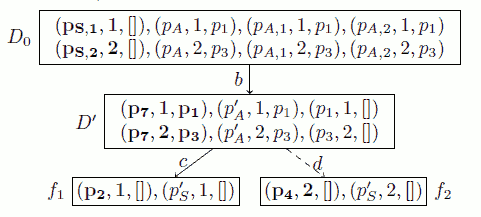
\includegraphics[scale=0.5]{5_4}
\par
Po przewidywaniu bc, DFA posiada stany $D_0$, $D'$, i $f_1$. Ze stanu $D'$ DFA,
\textit{closure} dochodzi do końca A i pobiera ze stosów $\Gamma$, wracając do stanów ATN w S.
Stan $f_1$ jednoznacznie przewiduje numer produkcji na 1. Stan f2 zostaje utworzony i podłączony do DFA
(wskazany przerywaną strzałką) podczas przewidywania drugiej frazy bd.
Funkcja \textit{adaptivePredict} najpierw używa symulacji DFA, aby dojść do $D'$ z $D_0$ względem b.
Przed zobaczeniem bd, $D'$ nie posiada żadnych krawędzi d, tak więc \textit{adaptivePredict}
musi użyć symulacji ATN, aby dodać krawędź $D' \overset{d}{\rightarrow}f_2$


\section{Rezultaty teoretyczne}
Ta sekcja identyfikuje kluczowe twierdzenia ALL(*) i pokazuje złożoność czasową parsera.
Zobacz Dodatek A dla dokładnych dowodów.
\\
\textbf{Twierdzenie 6.1}. (Poprawność). Parser ALL(*) dla nie-lewostronnie-rekurencyjnej
G rozpoznaje zdanie w wtedy i tylko wtedy gdy w $\in$ L(G).
\\
\textbf{Twierdzenie 6.2}. Języki ALL(*) są zamknięte ze względu na unię
\\
\textbf{Twierdzenie 6.3}. Parsowanie ALL(*) n symboli ma złożoność czasową O(n4)
\\
\textbf{Twierdzenie 6.4}. GSS ma O(n) węzłów dla n symboli wejściowych.
\\
\textbf{Twierdzenie 6.5}. Dwufazowy parsing dla nie-lewostronnie-rekurencyjnej G rozpoznaje
zdanie w wtedy i tylko wtedy gdy w $\in$ L(G).

\section{Rezultaty empiryczne}
Wykonaliśmy eksperymenty aby porównać wydajność parserów Java ALL(*) z
innymi strategiami do zbadania wydajności ALL(*) dla różnorodnych innych języków,
do podkreślenia efektu lookahead DFA cache na prędkość parsowania, i do dostarczenia
dowodu linowej wydajności ALL(*) w praktyce.

\subsection{Porównanie prędkości ALL(*) do innych parserów}
\begin{figure}[h]
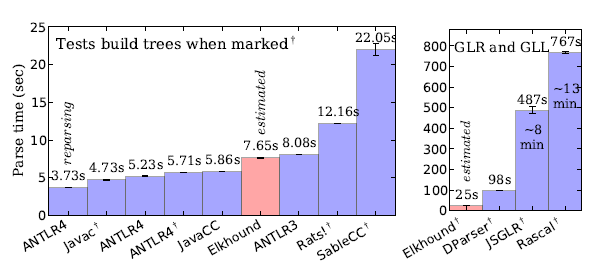
\includegraphics[scale=0.67]{Figure9.png}
\caption{
Porównanie Java czasu parsowania dla 10 narzędzi i 8 strategii na
bibliotece Java 6 i źródłach kompilatora (mniejsze wartości oznaczają szybciej).
12'920 plików, 3.6M linii, wielkość 123M.
Opis narzędzia zawiera: “tool name version [strategy].” ANTLR4 4.1 [ALL(*)]; Javac
7 [ręcznie zbudowany parser zejść rekurencyjnych i pierwszeństwa dla wyrażeń];
JavaCC 5.0 [LL(k)]; Elkhound 2005.08.22b [GLR] (testowany na Windows); ANTLR3 3.5 [LL(*)];
Rats! 2.3.1 [PEG]; SableCC 3.7
[LALR(1)]; DParser 1.2 [GLR]; JSGLR (z Spoofax) 1.1 [GLR];
Rascal 0.6.1 [GLL]. Testy uruchomione 10x z obfitą pamięcią, średnia/stddev
obliczona dla ostatnich 8 do uniknięcia kosztu JIT. Słupki błędów są znikome
ale pokazują pewne niestałości z powodu działania garbage collectora.
Aby uniknąć logarytmicznej skali, użyliśmy oddzielnego obrazka dla czasu parsowania GLR, GLL.
}
\end{figure}

\begin{figure}[h]
\begin{tabular}{|r||r|r|}
\hline
Tool & Time & RAM(M)\\
\hline\hline
$Javac^t$ & 89 ms & 7 \\
\hline
ANTLR4 & 201 ms & 8 \\
\hline
JavaCC & 206 ms & 7 \\
\hline
$ANTLR4^t$ & 360 ms  & 8 \\
\hline
ANTLR3 & 1048 ms &  143\\
\hline
$SableCC^t$ & 1'174 ms & 201 \\
\hline
$Rats!^t$ & 1'365 ms & 22 \\
\hline
$JSGLR^t$ & 15.4 sec & 1'030 \\
\hline
$Rascal^t$ & 24.9 sec & 2'622 \\
\hline
(no DFA) ANTLR4 & 42.5 sec & 27 \\
\hline
$elkhound^a$ & 3.35 min & 3 \\
\hline
$DParser^t$ & 10.5 hours & 100+ \\
\hline
$elkhound^t$ & out of mem & 5390+ \\
\hline
\end{tabular}
\caption{Czas i pamięć użyta do parsowania i opcjonalnego budowania drzew dla
3.2M pliku Java. Rozmiar pamięci jest medianą podawaną po GC podczas parsowania używając
-XX:+PrintGC opcji (dla C++ process monitoring). Czasy obejmują lexing; all input preloaded.
$^t$ Budowanie drzew; $^a$ Niejednoznaczność podczas parsowania, bez drzew}
\end{figure}

Nasz pierwszy eksperyment porównuje prędkość parsowania Java przez 10 narzędzi
i 8 strategii parsowania: ręcznie-wyregulowany zejść rekurencyjnych
z parsowaniem pierwszeństwa, LL(k), LL(*), PEG, LALR(1), ALL(*)
GLR, i GLL. Rysunek 9 pokazuje czas dla każdego narzędzia parsowania
12'920 plików źródłowych biblioteki Javy 6 i kompilatora.
Wybraliśmy Javę ponieważ miała ona najbardziej dostępną gramatykę wśród narzędzi
i przykładowe źródła Javy są obfite.
Gramatyki Java użyte w eksperymencie przyszły bezpośrednio z powiązanymi narzędziami
z wyjątkiem DParser i Elkhound, które nie oferowały odpowiedniej gramatyki Javy.
Przenieśliśmy gramatykę Java ANTLR do meta-składni tych narzędzi używając
jednoznacznych reguł wyrażeń arytmetycznych. Również osadzone akcje merge w
gramatyce Elkhound do ujednoznacznienia podczas parsowania do imitacji
rozdzielczości ANTLR w niejednoznaczności. Wszystkie pliki input były
ładowane do RAM przed parsowaniem i czasy odzwierciedlają średni czas obliczony
przez 10 całkowitych przejść korpusu, opuszczając dwa pierwsze dla
upewnienia się że nie mamy do czynienia z rozgrzewką kompilatora JIT.
Dla ALL(*) użyliśmy dwufazowego parsowania z Sekcji 3.2.
Testową maszyną był 6 core 3.33Ghz 16G RAM Mac OS X 10.7 desktop mający uruchomioną
Java 7 virtual machine. Elkhound and DParser parsers were
implemented in C/C++, które nie miały garbage collectora biegnącego równolegle.
Elkhound był ostatnio uaktualniony w 2005 roku
i dłużej nie był bufowany na Linuxie czy OS X, ale byliśmy w stanie zbudować go na
Windows 7 (4 core 2.67Ghz 24G RAM). Elkhound również mógł jedynie czytać z
pliku tak że Elkhound czas parsowania jest nieporównywalny.
W wysiłku by kontrolować prędkość maszyny różnice RAM kontra SSD, obliczyliśmy
współczynnik naszej Java test rig na naszej maszynie OS X czytającej z RAM do
ANTLR4
Javac
ANTLR4
ANTLR4
JavaCC
Elkhound
ANTLR3
Rats!
SableCC
5 0
10
15
20
25
Parse time (sec)
3.73s 4.73s 5.23s 5.71s 5.86s
7.65s 8.08s
12.16s
22.05s
estimated
reparsing
Tests build trees when marked
Elkhound
DParser
JSGLR
Rascal
0
100
200
300
400
500
600
700
800
25s
98s
487s
767s
GLR and GLL
estimated
~13
min
~8
min
test rig uruchomiony pod Windows z SSD. Nasze czasy Elkhound są w czasie Windows
pomnożonym przez współczynnik OS X do Windows.
\par
Dla tego eksperymentu, ALL(*) wyprzedza inne generatory parserów i jest
jedynie 20% wolniejszy niż parser zbudowany ręcznie w Javie. Kiedy porównywanie
uruchomione z konstrukcją drzewa (oznaczone przez † na Rysunku 9), ANTLR 4 jest
około 4.4x szybszy niż Elkhound, najszybsze narzędzie GLR które testowaliśmy,
i 135x szybsze niż GLL (Rascal). ANTLR 4 is niedeterministyczny ALL(*) parser
był nieco szybszy niż JavaCC’s deterministyczny LL(k) parser i około
2x szybszy niż Rats!’s PEG. W oddzielnym teście, wyszło że ten ALL(*)
wyprzedza Rats! Na jego własnej gramatyce PEG konwertowanej na składnięANTLR
(8.77s vs 12.16s).
Parser LALR(1) nie wykonywał dobrze przeciw narzędziom LL ale on mógłby
być SableCC’s implementacją a nie niedociągnięcie LALR(1). (Gramatyka Java z JavaCUP,
inny narzędzie LALR(1), było niekompletne i nie mogło parsować korpusu.)
Kiedy reparsowaliśmy korpus, ALL(*) lookahead z powodu trafień cache jest
szybsze 3.73s. Kiedy reparsowaliśmy z konstrukcją drzewa (czas nie pokazany),
ALL(*) pokonał ręcznie budowane Javac (4.4s kontra 4.73s).
Prędkość ponownego parsowania jest kwestią dla narzędzi takich jak środowisko deweloperskie.
\par
Parsery GLR które testowaliśmy są nawet o dwa rzędy wielkości wolniejsze w
parsowaniu Javy niż ALL(*). Z narzędzi GLR,
Elkhound ma najlepszą wydajność ponieważ polega on na liniowym stosie
LR(1) zamiast GSS gdzie możliwe.
Dalej, pozwoliliśmy Elkhound pozbyć się niejednoznaczności podczas
parsowania jak ALL(*). Elkhound używa oddzielnego lexera, w odróżnieniu od
JSGLR i DParser, które nie mają skanera.
Możliwe wyjaśnienie dla obserwowanej różnicy wydajności z ALL(*) jest
ze gramatykę Java przenieśliśmy do Elkhound i Dparser jest
stronniczy w kierunku ALL(*), ale ten zarzut nie jest zasadny.
GLR powinien także korzystać z wysoko deterministycznej i jednoznacznej gramatyki.
GLL było najwolniejsze w tym teście może dlatego że zespół Rascala przeniósł SDF GLR gramatykę Java,

a
Ujednoznacznienie poprzez parsowanie, bez drzew, szacowany czas.
Który jest nie optymalizowany dla GLL (wariacje gramatyki mają wpływ na wydajność.)
Rascal jest również bez skanera i jest obecnie jedynym dostępnym narzędziem GLL.
\par
Największym problemem z generalnymi algorytmami jest to że one są wysoko nieprzewidywalne
jeśli chodzi o czas i pamięć, które mogą czynić je nieodpowiednie dla
niektórych komercyjnych aplikacji. Obrazek 10 podsumowuje wydajność tych
samych narzędzi z pojedynczym plikiem Java 3.2M. Elkhound wzięte 7.65s do parsowania 123M Java
korpus, ale wzięte 3.35 minuty do parsowania pliku Java 3.2M. Spowodował on
błąd (out of memory) z konstrukcją lasu parsowania.
Czas DParsera skoczył z czasu korpusu 98s do 10.5 godzin.
na pliku 3.2M file. Prędkość Rascala JSGLR skalowały się miarę dobrze do 3.2M pliku,
ale użyły 2.6G and 1G RAM, odpowiednio.
W przeciwieństwie, ALL(*) parsował plik 3.2M w 360ms z konstrukcją drzewa używając 8M.
ANTLR 3 jest szybki ale jest wolniejszy i używa więcej pamięci (z powodu wstecznego pamiętania) niż ANTLR 4.

\subsection{Wydajność ALL(*) ze względu na języki}
\begin{figure}[h]
\begin{tabular}{|l||r|}
\hline
Grammar & KB/sec \\
\hline\hline
XML & 45'993 \\
Java & 24'972 \\
JSON & 17'696 \\
DOT & 16'152 \\
Lua & 5'698 \\
C & 4'238 \\
Verilog2001 & 1'994 \\
Erlang &751 \\
\hline
\end{tabular}
\caption{Wydajność w
KByte/sec. Lexing+parsing;
cały wejście załadowane do RAM.}
\end{figure}

\begin{figure}[h]
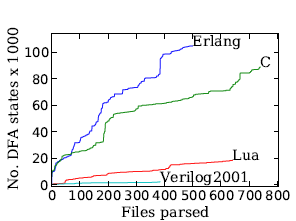
\includegraphics[scale=0.8]{Figure12.png}
\caption{
Tempo wzrostu DFA vs ilość parsowanych plików.
Pliki parsowane w kolejności w jakiej były na dysku.
}
\end{figure}

Obrazek 11 podaje wydajność w bajtach na sekundę wszystkich parserów ALL(*)
dla 8 języków włączając w to Javę dla porównania. Ilość plików testowych
i rozmiary plików różnią się znacznie (według wejścia które mogliśmy rozsądnie zebrać);
mniejsze pliki uzyskują wyższą wariancję czasu parsowania.
\begin{itemize}
\item C Pochodzi ze specyfikacji C11; nie ma pośredniej lewej rekursji,
zmieniona reguła wrażliwa na stos aby  wykonać SLL (zobacz tekst poniżej): 813
preprocesowanych plików, 159.8M źródeł z bazy postgres.
\item Verilog2001 Pochodzi z specyfikacji Verilog 2001, usunięta pośrednia lewa rekursja:
385 plików, 659k z [3] i internetu.
\item JSON Pochodzi ze specyfikacji. 4 pliki, 331k z twittera.
\item DOT: Pochodzi ze specyfikacji. 48 plików,19.5M zebranych z internetu.
\item Lua: Pochodzi ze specyfikacji Lua 5.2. 751 plików, 123k z githuba.
\item XML Pochodzi ze specyfikacji. 1 plik, 117M z XML benchmark.
\item Erlang Pochodzi z gramatyki LALR(1). 500 preprocesowanych plików, 8M.
\end{itemize}
Niektóre z tych gramatyk mają wydajność rozsądną ale dużo wolniejszy czas parsowania w
porównaniu do Javy i XML ale demonstrują że programiści mogą konwertować język
specyfikacji do ANTLR meta-składni
i dostać działającą gramatykę bez dużej modyfikacji.
(W naszym doświadczeniu specyfikacje gramatyki są rzadko dostrajane do szczeólnych narzędzi lub strategii parsowania i są często niejednoznaczne.) Później, programiści mogą użyć profilowania ANTLR i diagnostyki do polepszenia wydajności tak jak inne programistyczne zadanie.
Dla przykładu, specyfikacja gramatyki C11 jest LL nie SLL
z powodu reguły declarationSpecifiers, która zmieniliśmy aby była SLL w naszej gramatyce C (dostając 7x przeypieszenia prędkości).

\subsection{Oddziaływanie lookahead DFA na wydajność}
Lookahead DFA cache jest krytyczne gdy chodzi o wydajność ALL(*).
Aby zademonstrować odziaływanie cache na prędkość parsowania, zablokowaliśmy DFA
i powtórzyliśmy nasze eksperymenty z Javą.
Rozważmy czas parsowania 3.73s z Obrazka 9 reparsowania korpusu Javy z czystymi
trafieniami w cache.
Z zablokowanym zupełnie lookahead DFA cache, parserowi zajmowało to 12 minut (717.6s).
Obrazek 10 pokazuje że zablokowanie cache zwiększa czas parsowania z 203ms do 42.5s na 3.2M pliku.
Ta wydajność jest zgodna z wysokim kosztem parserów GLL i GLR które również nie redukują
spekulacji przez zapamiętywanie decyzji parsera.
Jako pośrednia wartość, czyszczenie cache DFA przed parsowaniem każdego pliku
korpusu powoduje że całkowity czas wynosi 34s zamiast 12 minut.
To izoluje użycie cache do jednego pliku i demonstruje żet rozgrzewka cache
zdarza się szybko nawet przy pojedynczym pliku.
\par
Wielkość DFA zwiększa się liniowo gdy parser napotyka nowe frazy lookahead.
Obrazek 12 pokazuje wzrost ilości stanów DFA jak (najwolniejsze cztery) parsery z Obrazka 11
napotyka nowe pliki. Języki jak C które są skonstruowane z
wspólną lewy-prefix wymaga głębokiego lookahead w LL parserach do
rozróżnienia fraz; np. struct {...} x; i struct {...}f(); dzielą wielki lewy-prefiks.
W przeciwieństwie Verilog2001 parser używa bardzo mało stanów DFA
(ale działa wolniej z powodu reguły nie SLL). Podobnie, po przejrzeniu całego 123M korpusu Java,
Java parser używa właśnie 31'626 stanów DFA, dodając średnio  ˜2.5 stanu na parsowany plik.
Wielkość DFA jednak rośnie gdy parser napotyka nieznane wejście.
Programiści mogą czyścić cache i ALL(*) zaadaptuje się do kolejnego wejścia.

\subsection{Empiryczna złożoność czasowa parsowania}
Biorąc pod uwagę szeroki zakres wydajności na Rysunku 11, można by posądzać o nieliniowe
zachowanie dla wolniejszych parserów. Aby prześledzić, wykreślimy czas parsowania według
wielkości pliku na Rysunku 13 i narysujemy regresję najmniejszych kwadratów
i krzywej dopasowania danych LOWESS [6].
\begin{figure}[h]
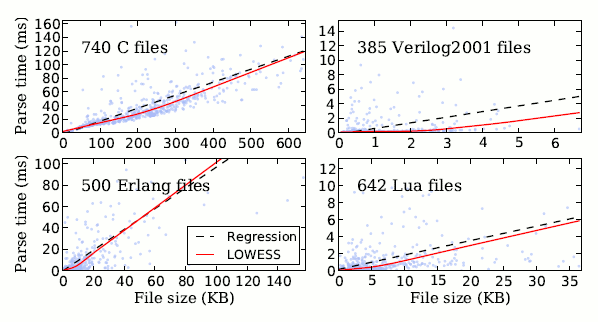
\includegraphics[scale=0.67]{Figure13.png}
\caption{
Liniowy czas pasowania vs wielkość pliku. Regresja liniowa (linia przeywana)
i nieskrępowana krzywa LOWESS zbiegają się dając silny dowód liniowości
Krzywe obliczone na (dolne) 99\% weilkości plików ale powiększone
aby pokazać szczegóły dolnego 40\% czasu parsowania.
}
\end{figure}
Krzywe LOWESS są parametrycznie nieskrępowane (nie wymagane aby były linią lub
jakimś szczególnym wielomianem) i one wirtualnie odzwierciedlają każdą
linię regresji, dostarczając silnego dowodu że relacja
pomiędzy czasem parsowania a wielkością wejścia jest liniowa.
Ta sama metodologia pokazuje że parser wygenerowany z gramatyki nie-SLL (nie pokazane)
wzięty ze specyfikacji C11 jest również liniowy, pomimo że dużo wolniejszy niż nasza wersja SLL.
\par
Powinniśmy jeszcze zobaczyć nieliniowe zachowanie w praktyce ale teoretyczne
zachowanie najgorszego przypadku parsowania ALL(*) jest O($n^4$). Eksperymentalne
dane czasu parsowania dla następującej wymyślonej gramatyki najgorszego przypadku
wykazuje zachowanie czwartego stopnia dla wejścia a, aa, aaa,
..., $a^n$ (z n $\leqslant$ 120 symboli mogliśmy przetestować w rozsądnym czasie).
//
S $\rightarrow$ A, A $\rightarrow$ aAAj|aA|a.
//
Generowany parser wymaga predykcji na każdym symbolu wejściowym
i każda predykcja musi badać cały pozostały input.
Operacja closure wykonana dla każdego symbolu unput musi badać
całą głębokość GSS, która może być rozmiaru n, Ostatecznie, łączenie
dwóch GSS może zająć O(n) w naszej implementacji, dając
złożoność O($n^4$).
\par
Z naszych eksperymentów otrzymaliśmy że przeniesienie analizy gramatyki
do czasu parsowania do dania ALL(*) siły jest nie tylko praktyczne
ale daje ekstremalnie wydajne parsery, rywalizujące z
ręcznie dostrajanymi rekurencyjnymi parserami kompilatora Javy.
Pamiętanie rezultatów analizy w DFA jest krytyczne do takiej wydajności.
Mimo teoretycznej złożoności O($n^4$), w praktyce ALL(*) zdaje się by liniowe
i nie wykazuje nieprzewidzianego zachowania jeśli chodzi o czas lub
pamięć jak ogólne algorytmy.


\section{Powiązane prace}
Przez dekady pracowano w kierunku zwiększenia
siły rozpoznawania recognition wydajnych ale nie ogólnych
parserów LL i LR i zwiększenia wydajności ogólnych algorytmów
Earleya O(n3) [8]. Parr [21] i Charles [4] statystycznie generowane parsery LL(k) i LR(k)
dla k > 1. Parr i Fisher’s LL(*) [20] i Bermudez i Schimpf’s LAR(m) [2]
statystycznie liczone parsery LL i LR wzbogacone o cykliczny
DFA który mógł badać dowolną ilość podglądanych symboli. Te
parsery bazowały na parserach LL-regular [12] i LR-regular [7]
które miały niepożądaną właściwość bycia nierozstrzygalnym w ogólności.
Wprowadzenia algorytmu z nawrotami(backtrackingu) dramatycznie zwiększyło się rozpoznawania
i uniknięto kwestii nierozstrzygalności statycznej analizy gramatyki
ale jest niepożądane ponieważ osadzone mutatory redukowały wydajność
i komplikowały debugowanie krok po kroku. parsery Packrat (PEGs) [9] próbowały decyzji
produkcji w kolejności I wybierały pierwszą która dawała sukces. PEG są
O(n) ponieważ one pamiętają częściowy rezultat parsowania ale cierpią
na aberrację a | ab gdzie ab jest milcząco nie brane pod uwagę.
\par
Aby zwiększyć ogólną wydajność parsowania, Tomita [26] wprowadził GLR, ogólny algorytm
bazujący na LR(k) który konceptualnie forkuje subparsery dla każdego stanu
LR(k) z konfliktem w czasie parsowania to badania wszystkich możliwych ścieżek.
Tomita pokazuje że GLR jest 5x-10x szybszy niż Earley. Kluczowy komponent
parsowania GLR jest graph-structured stack (GSS) [26] który zapobiega parsowaniu
tego samego wejścia dwukrotnie w ten sam sposób.
(GLR wkłada symbole wejściowe i stany LR na GSS podczas gdy ALL(*) wkłada stany ATN)
Elkhound [18] wprowadził hybrydowe parsery GLR które używają pojedynczy stos
dla wszystkich decyzji LR(1) a GSS kiedy niezbędne jest dopasowanie
niejednoznacznych porcji wejścia. (Zobaczyliśmy że parsery Elkhounda
są szybsze niż inne GLR.) GLL [25] jest analogiem LL parserów GLR
i również używa subparserów i GSS do badania wszystkich możliwych ścieżek;
GLL używa lookahead k = 1 gdzie można dla wydajności.
GLL jest O(n3) a GLR jest O(np+1)
gdzie p jest długością najdłuższej produkcji gramatyczne.
\par
Parsery Earleya skalują się dobrze od  O(n) dla deterministycznych gramatyk
do O(n3) dla niejednoznacznych gramatyk ale wydajność
nie jest dość dobra w ogólnym użyciu.
LR(k) maszyny stanów mogą polepszyć wydajność takich parserów
prze statystyczne obliczanie tak dużo jak to możliwe. LRE [16] jest jednym
takim przypadkiem. Mimo tych optymizacji ogólne algorytmy pozostają
bardzo wolne w porównaniu do deterministycznych parserów wzbogaconych
o głęboki podgląd symboli.
\par
Problem z dowolną liczbą podglądanych symboli jest taki że jest niemożliwe
wyliczyć statystycznie dla wielu użytecznych gramatyk (warunek LLregular jest nierozstrzygalny.) Przez przeniesienie analizy podglądanych symboli do czasu analizy ALL(*) zdobył siłę do obsługi jakiejkolwiek gramatyki bez lewostronnej rekurencji ponieważ może uruchomić subparsery do określenia jaka ścieżka prowadzi to poprawnego parsowania. Inaczej niż GLR,
spekulacja zatrzymuje się kiedy wszystkie pozostałe subparsery są powiązane z pojedynczą alternatywą a produkcji, tak więc wyliczając minimalną sekwencję podglądanych symboli.. Aby zyskać wydajność, ALL(*) zapamiętuje mapowanie z tej sekwencji lookahead to przewidzianej produkcji używając DFA dla użycia przez kolejne decyzje.
Podzbiory języka bezkontekstowego napotykane podczas parsowania są skończone i dlatego języki ALL(*) lookahead są regularne.
Ancona et al [1] również wykonują analizę czasu parsowania ale oni
jedynie obliczają stały lookahead LR(k) i nie adaptują do faktycznego wejścia jak to robi ALL(*).
Perlin [23] działa na RTN jak ALL(*) ale oblicza  lookahead k = 1 podczas parsowania.
\par
ALL(*) jest podobne do Earley w tym że obydwa są top-down i
operują na reprezentacji gramatyki w czasie parsowania ale
Earley parsuje nie licząc lookahead DFA. W tym sensie,
Earley nie wykonuje analizy gramatycznej, Earley również nie zarządza jawnie
GSS podczas parsowania. Zamiast tego element w stanach Earleya
mają “wskaźniki rodzica” które odnoszą się do innych stanów
kiedy są w wątku razem
Operacja SCANNER Earleya
koresponduje do funkcji ALL(*) move. Operacje PREDICTOR i COMPLETER
korespondują do push i pop in funkcji closure ALL(*)
Stan Earleya jest zbiorem wszystkich konfiguracji parsera osiągalnych
w pewnej absolutnej głębokości wejścia podczas gdy stan DFA ALL(*) jest zbiorem konfiguracji
osiągalnych z głębokości podglądu relatywnej do bieżącej decyzji
Inaczej niż w kompletnie ogólnych algorytmach, ALL(*) wyszukuje
pojedyncze parsowanie wejścia, które pozwala użyć wydajnego stosu LL podczas parsowania.
\par
Strategie parsowania które ciągle spekulują lub wspomagają niejednoznaczność
mają trudności z mutatorami ponieważ ciężko wtedy o cofnięcie działania.
Brak mutatorów redukuje ogólność semantycznych predykatów które zmieniają parsowanie ponieważ nie można testować dowolnie stanu obliczonego wcześniej podczas parsowania.
Rats! [10] wspomaga ścisłe semantyczne predykaty a Yakker [13] wspomaga
semantyczne predykaty które są funkcjami poprzednio parsowanych symboli terminalnych.
Ponieważ ALL(*) nie spekuluje podczas faktycznego parsowania, wspomaga dowolne mutatory i semantyczne predykaty..
Miejsce wyklucza bardziej szczegółowe dyskusje o powiązanych pracach; bardziej szczegółowa analiza może być znaleziona w [20].

%+Bibliography
\begin{thebibliography}{99}
\bibitem{Label1}ANCONA, M., DODERO, G., GIANUZZI, V., AND MORGAVI,
M. Efficient construction of LR(k) states and tables. ACM
Trans. Program. Lang. Syst. 13, 1 (Jan. 1991), 150–178
\bibitem{Label2}BERMUDEZ, M. E., AND SCHIMPF, K. M. Practical arbitrary
lookahead LR parsing. Journal of Computer and System Sciences
41, 2 (1990).
\bibitem{Label3}BROWN, S., AND VRANESIC, Z. Fundamentals of Digital Logic
with Verilog Design. McGraw-Hill series in ECE. 2003.
\bibitem{Label4}CHARLES, P. A Practical Method for Constructing Efficient
LALR(k) Parsers with Automatic Error Recovery. PhD thesis,
New York University, New York, NY, USA, 1991.
\bibitem{Label5}CLARKE, K. The top-down parsing of expressions. Unpublished
technical report, Dept. of Computer Science and Statistics,
Queen Mary College, London, June 1986.
\bibitem{Label6}CLEVELAND, W. S. Robust Locally Weighted Regression and
Smoothing Scatterplots. Journal of the American Statistical
Association 74 (1979), 829–836.
\bibitem{Label7}COHEN, R., AND CULIK, K. LR-Regular grammars—an extension
of LR(k) grammars. In SWAT ’71 (Washington, DC, USA,
1971), IEEE Computer Society, pp. 153–165.
\bibitem{Label8}EARLEY, J. An efficient context-free parsing algorithm. Communications
of the ACM 13, 2 (1970), 94–102.
\bibitem{Label9}FORD, B. Parsing Expression Grammars: A recognition-based
syntactic foundation. In POPL (2004), ACM Press, pp. 111–122.
\bibitem{Label10}GRIMM, R. Better extensibility through modular syntax. In
PLDI (2006), ACM Press, pp. 38–51.
\bibitem{Label11}HOPCROFT, J., AND ULLMAN, J. Introduction to Automata Theory,
Languages, and Computation. Addison-Wesley, Reading,
Massachusetts, 1979.
\bibitem{Label12}JARZABEK, S., AND KRAWCZYK, T. LL-Regular grammars.
Information Processing Letters 4, 2 (1975), 31 – 37.
\bibitem{Label13}JIM, T., MANDELBAUM, Y., AND WALKER, D. Semantics and
algorithms for data-dependent grammars. In POPL (2010).
\bibitem{Label14}JOHNSON, M. The computational complexity of GLR parsing.
In Generalized LR Parsing, M. Tomita, Ed. Kluwer, Boston,
1991, pp. 35–42.
\bibitem{Label15}KIPPS, J. Generalized LR Parsing. Springer, 1991, pp. 43–59.
\bibitem{Label16}MCLEAN, P., AND HORSPOOL, R. N. A faster Earley parser. In
CC (1996), Springer, pp. 281–293.
\bibitem{Label17}MCPEAK, S. Elkhound: A fast, practical GLR parser generator.
Tech. rep., University of California, Berkeley (EECS), Dec.
2002.
\bibitem{Label18}MCPEAK, S., AND NECULA, G. C. Elkhound: A fast, practical
GLR parser generator. In CC (2004), pp. 73–88.
\bibitem{Label19}MCPEAK, S., AND NECULA, G. C. Elkhound: A fast, practical
GLR parser generator. In CC (2004), pp. 73–88.
\bibitem{Label20}PARR, T., AND FISHER, K. LL(*): The Foundation of the
ANTLR Parser Generator. In PLDI (2011), pp. 425–436.
\bibitem{Label21}PARR, T. J. Obtaining practical variants of LL(k) and LR(k)
for k > 1 by splitting the atomic k-tuple. PhD thesis, Purdue
University, West Lafayette, IN, USA, 1993.
\bibitem{Label22}PARR, T. J., AND QUONG, R. W. Adding Semantic and Syntactic
Predicates to LL(k)—pred-LL(k). In CC (1994).
\bibitem{Label23}PERLIN, M. LR recursive transition networks for Earley and
Tomita parsing. In Proceedings of the 29th Annual Meeting
on Association for Computational Linguistics (1991), ACL ’91,
pp. 98–105.
\bibitem{Label24}PLEVYAK, J. DParser: GLR parser generator, Visited Oct. 2013.
\bibitem{Label25}SCOTT, E., AND JOHNSTONE, A. GLL parsing. Electron. Notes
Theor. Comput. Sci. 253, 7 (Sept. 2010), 177–189.
\bibitem{Label26}TOMITA, M. Efficient Parsing for Natural Language. Kluwer
Academic Publishers, 1986.
\bibitem{Label27}WOODS, W. A. Transition network grammars for natural language
analysis. Comm. of the ACM 13, 10 (1970), 591–606.
\end{thebibliography}
%-Bibliography
\appendix
\section{Analiza poprawności i złożoności}
\textbf{Twierdzenie A.1.} Języki ALL(*) są zamknięte w unii.
\\ \\
Dowód. Niech predykowalne gramatyki $G_1 = (N_1, T, P_1, S_1, \Pi_1,\mathcal{M}_1)$
i $G_2 = (N_2, T, P_2, S_2, \Pi_1,\mathcal{M}_1)$ opisują odpowiednio L($G_1$) i L($G_2$).
Dla stosowalności zarówno do parserów jak i parserów bezskanerowych
przyjmijmy że przestrzeń terinali T jest zbiorem poprawnych znaków.
Przyjmijmy że  $N1 \cap N2 = \varnothing$ przez przezwanie nieterinali
w razie potrzeby.
Przyjmijmy że predykaty i mutatory $G_1$ i
$G_2$ działają w rozłącznych środowiskach $S_1$ and $S_2$.
Konstruujmy:
\\ \\
$G' = (N_1 \cup N_2, T, P_1 \cup P_2, S',\Pi_1 \cup \Pi_2,\mathcal{M}_1 \cup \mathcal{M}_2)$
\\ \\
z S' = $S_1 | S_2$. Wtedy L(G') = $L(G_1) \cup L(G_2)$.
\\ \\
\textbf{Lemat A.1.} Parser ALL(*) dla nie lewostronnie rekurencyjnej G z
deaktywowanym lookahead DFA rozpoznaje zdanie wtedy i tylko wtedy gdy  $w \in L(G)$.
\\ \\
Dowód. ATN dla G rozpoznaje $w$ wtedy i tylko wtedy gdy $w \in L(G)$.
Dlatego możemy równoważnie dowieść że ALL(*) jest
wierną implementacją ATN. Bez lookahead DFA predykcja jest
prostą symulacją ATN: zstępujący parser który podejmuje
dokładne decyzje parsowania używając GLR-podobnych podparserów które
mogą badać cały pozostały input i wołanie stosu podmaszyn ATN.
\\ \\
\textbf{Twierdzenie A.2.} (Poprawność). Parser ALL(*) dla nie lewostronnie
rekurencyjnej G rozpoznaje zdanie $w$ wtedy i tylko wtedy gdy $w \in L(G)$.
\\ \\
Dowód. Lemat A.1 pokazuje że parser ALL(*) poprawnie rozpoznaje
$w$ bez cache DFA. Istotą dowodu
następnie jest pokazać że adaptywny lookahead ALL(*) DFA nie
psuje parsowania dając inną decyzję predykcji niż
prosta symulacja ATN. Potrzebujemy jedynie rozważyć
przypadek nieprzewidującego parsingu SLL jak ALL(*)
jedynie only buforuje w cache rezulaty decyzji w tym przypadku.
\par
przypadek "wtedy": Przez indukcję na stanie lookahead DFA dla
dowolnie danej decyzji A. Przypadek podstawowy.
Pierwsza predykcja dla A zaczyna się
pustym DFA i musi aktywować symulację ATN do
wybrania alternatywy $\alpha_i$ używając prefisku $u \preceq w_r$.
Skoro symulacja ATN
daje właściwe przewidywania, parser ALL(*) poprawnie przewiduje
$\alpha_i$ na starcie i następnie zapisuje mapowanie u : i
w DFA. Jeśli jest tam pojedyncza wykonalna alternatywa, $i$ jest
związanym z nią numerem produkcji.
Jeśli symulacja znajduje ATN wiele wykonalnych alternatyw,
i jest minimalnym numerem produkcji związanych
z alternatywami z tego zbioru.
\par
Krok indukcji. Przyjmijmy że lookahead DFA poprawnie przewiduje
produkcje dla każdego prefiksu $u$ z $w_r$ widzoanego przez parser
w A. Muismy pokazać że startując z istniejaćego DFA, ALL(*)
właściwie doda ścieżkę przez DFA dla nieznanego prefiksu $u$
z $w'_r$. Mamy kilka przypadków:
\begin{enumerate}
\item $u \preceq w'_r$ i $u \preceq w_r$ dla poprzedniego $w_r$.
Lookahead DFA daje poprawną odpowiedź dla $u$ przez założenie indukcyjne.
DFA jest nie uaktualniane.
\item $w'_r = bx$ i wszystkie poprzednie $w_r = ay$ dla pewnego $a \neq b$.
Ten przypadek redukuje się do podstawoewego przypadku zimnego startu
ponieważ nie mam tam krawędzi
$D_0 \overset{b}{\rightarrow}D$.
Symulacja ATN przewiduje $\alpha_i$ i ododaje ściężkę
dla $u \preceq w'_r$ z $D_0 do f_i$.
\item $w'_r = vax$ i $w_r = vby$ dla pewnego poprzednio widzianego
$w_r$ ze wspólnym prefiksem $v$ i $a \neq b$.
Symulacja DFA osiągnie D z $D_0$ dla wejścia v.
D ma krawędź dla $b$ ale nie $a$.
Symulacja ATN przewidzi $\alpha_i$ i wzbogaci DFA, startując z
krawędzi na $a$ z $D$ prowadząc ostatecznie do $f_i$.
\end{enumerate}
\par
przypadek "tylko wtedy": Parser ALL(*) zgłasza błąd składni dla
$w \notin L(G)$. Przyjmijmy odwrotnie, że parser z sukcesem
parsuje $w$. To pociąga za sobą że istnieje sekwencja wyprowadzająca
konfigurację ATN
$(\mathbb{S}, p_S, [], w) \rightarrow_* (\mathbb{S}, p'_S, [], \epsilon)$
dla $w$
przez odpowiadajcy G ATN. Ale to wymagało by $w \in
L(G)$, z Definicji ??. Dlatego parser ALL(*) zgłasza
błąd składni dla w. Dokładność lookahead cache ALL(*)
jest bez znaczenia ponieważ nie ma możliwej ścieżki przez ATN
lub parser.
\\ \\
\textbf{Lemat A.2.} Zbiór wykonalnych produkcji dla LL jest zawsze
podzbiorem wykonalnych produkcji SLL dla danej decyzji A i
pozostałego wejściowego ciągu $w_r$.
\\ \\
Dowód. Jeśli kluczowa operacja analizy move-closure nie
osiągnie stanu stop $p'_A$ dla podmaszyny A, SLL i LL postępują
identycznie i dzielą ten sam zbiór wykonalnych produkcji.
\par
Jeśli closure osiągnie stan stopu dla reguły wejściowej decyzji,
$p'_A$, tam są konfiguracje w formie $(p'_A, -, \gamma)$ gdzie,dla
wygody, zwykły GSS $\Gamma$ jest dzielony na pojedyncze stosy, $\gamma$. W
trybie predykcji LL, $\gamma = \gamma_0$, które jest bądź pojedynczym stosem lub
pustym jeśli A = S. W trybie SLL, $ \gamma = \#$, sygnalizując brak informacji
o stosie. Funkcja \textit{closure} musi rozważać wszystkie możliwe $\gamma_0$
wołania stosu parsera. Ponieważ jakikolwiek pojedynczy stos musi być zawarty
w zbiorze wszystkich możliwych wołań stosu, operacje LL closure
rozważają co najwyżej tę samą ilość ścieżek przez ATN co SLL.
\\ \\
\textbf{Lemat A.3.} Dla $w \notin L(G)$ i nie lewostronnie rekurencyjnej
G, SLL zgłasza błąd składni.
\\ \\
Dowód. Podobnie jak w przypadku "tylko wtedy" Twierdzenia 6.1, nie ma poprawnego
wyprowadzenia konfiguracji ATN dla $w$ bez względu jak adaptivePredict
wybierze produkcje.
\\ \\
\textbf{Twierdzenie A.3.} Dwustopniowe parsowanie dla nie lewostronnie rekurencyjnej
G rozpozna zdanie $w$ wtedy i tylko wtedy gdy $w \in L(G)$.
\\ \\
Dowód. Z Lematu A.3, SLL i LL zachowują się tak samo kiedy
$w \notin L(G)$. Pozostaje pokazać że predykcja SLL bądź
zachowuje się jak LL dla wejścia $w \in L(G)$ lub zgłasza błąd składni,
sygnalizując potrzebę drugiej fazy LL. Niech $\mathcal{V}$ i $\mathcal{V'}$ będą
zbiorami numerów wykonalnych produkcji dla A odpowiednio używając SLL i LL,
Z Lematu A.2, $\mathcal{V'} \subseteq \mathcal{V}$. Są dwa przypadki
do rozważenia:
\begin{enumerate}
\item If $min(\mathcal{V}) = min(\mathcal{V'})$, SLL i LL
wybierają tą samą produkcję.
SLL powiedzie się dla $w$. To jest, $\mathcal{V}$ = \{1, 2, 3\}
i $\mathcal{V'}$ =
\{1, 3\} or $\mathcal{V}$ = \{1\} i $\mathcal{V}$ = \{1\}.
\item If $min(\mathcal{V}) \neq min(\mathcal{V'})$ wtedy $min(\mathcal{V})
 \notin \mathcal{V]}$ ponieważ LL znajduje że
$min(\mathcal{V})$ jest niewykonalna. SLL powinien zgłosić błąd składni.
To jest, $\mathcal{V}$ = \{1, 2, 3\} i $\mathcal{V'}$ = \{2, 3\}
lub $\mathcal{V}$ = \{1, 2\} i $\mathcal{V'}$ = \{2\}.
\end{enumerate}
We wszystkich możliwych kombinacjach $\mathcal{V}$ i $\mathcal{V'}$,
SLL zachowuje się jak LL lub zgłasza błąd syntaktyczny dla $w \in L(G)$.
\\ \\
\textbf{Twierdzenie A.4.} GSS ma O(n) węzłów dla $n$ wejściowych symboli.
Dowód. Dla nieterminali N i stanów Q ATN jest |N| $\times$
|Q| $p\overset{A}{\rightarrow}q$ przejść ATN jeśli każda pozycja gramatyczna
wywoła każdy nieterminal. To limituje ilość nowych węzłów GSS
do $|Q|^2$ dla operacji closure (która nie może przejść
krawędzi terminalowych). ALL(*) wykonują n + 1 operacji closure dla n symboli
wejściowych dając $|Q|^2(n + 1)$ węzłów lub O(n) skoro Q nie jest
funkcją wejścia.
\\ \\
\textbf{Lemat A.4.} Złożoność czasowa badania symbolu lookahead wynosi O($n^2$).
\\ \\
Dowód. Lookahead jest operacją move-closure która wylicza
nowy docelowy stan DFA D' jako funkcję konfiguracji ATN
w D. Jest $|Q| \times m \approx |Q|^2$ konfiguracji postaci
(p, i, _) $\in$ D dla |Q| stanów ATN i $m$ alternatywnych
produkcji w bieżącej decyzji. Koszt move nie jest
funkcją rozmaru n wejścia. Closure D oblicza closure(c)
$\forall c \in D$ and closure(c) może przejść spowrotem
całe GSS do korzenia (pustego stosu). To daje koszt $|Q|^2$ konfiguracji
razy $|Q|2(n + 1)$ węzły GSS (z Twierdzenia A.4) lub O(n)
operacji dodawania by zbudować $D'$. Dodawanie konfiguracji jest dominujace
przez łączenie grafu, które (w naszej implementacji) jest proporcjonalne
do głębokości grafu. Całkowity koszt move-closure jest O($n^2$).
\\ \\
\textbf{Twierdzenie A.5.} Parsowanie ALL(*) n wejściowych symboli zajmuje
O($n^4$) czasu.
\\ \\
Dowód. W najgorszym przypadku parser musi badać wszystkkie pozostałe
symbole wejściowe podczas predykcji dla każdego z n wejściowych symboli
dając O($n^2$) operacji lookahead. Koszt każdej operacji lookahead
jest O($n^2$) z Lematu A.4 dając ogólny koszt parsowania O($n^4$).
\section{Pragmatyka}
Ta część opisuje pewne praktyczne rozważania
związane z implementacją algorytmu ALL(*).

\subsection{Redukowanie czasu rozgrzewki}
Dużo decyzji w gramatyce jest LL(1) i one są łatwe do identyfikacji
statycznie. Zamiast zawsze generować “przełącz się na
adaptivePredict” decyzje w rekurencyjnych zstępujących parserach,
ANTLR generuje decyzje “przełącz się na typ tokenu” gdziekolwiek
jest możliwe. Ta optymalizacja LL(1) nie wpływa na wielkość
generowanego parsera ale redukuje ilość lookahead DFA
które parser musi wyliczyć.
\par
Oryginalnie przeczuliśmy "trenowanie” parsera na wielkim
korpusie wejściowym a następnie zapisanie lookahead DFA na dysk
aby uniknąć jeszcze raz obliczania DFA dla kolejnych przebiegów parsera.
Jak pokazane w części 7, konstrukcja lookahead DFA jest wystarczająco szybka
tak że zapisanie i odczyt DFA jest zbyteczny.

\subsection{Wyliczenie semantycznych predykatów}
Dla jasności, algorytm opisany w tym artykule uźywa czystej
symulacji ATN dla wszystkich decyzji które mają that semantyczne predykaty
na lewymch krawędziach produkcji W praktyce ANTLR używa lookahead
DFA które śledzą predykaty i akceptują stany do obsługi senemtycznej
zależnej od kontekstu predykcji. Śledzenie predykatów w
DFA pozwala predykcjom uniknąć drogiej symulacji ATN jeśli
wyliczenie predykatu w ciągu symulacji SLL przewidzi unikalną
produkcję. Semantyczne predykaty nie są powszechne ale są krytyczne
do rozwiązywania pewnych zależnych od kontekstu problemów paroswania, to jest,
predykaty są używane wewnętrznie przez ANTLR do kodowania
priorytetu operatorów przy przepisywaniu lewostronnie rekurencyjnych reguł.
Tak że to jest warte dodatkowej złożoności do obliczenia
predykatów podczas predykcji SLL.
Rozważmy repdykowaną regułę z Części 2.1:
\par
id : ID | \{!enum_is_keyword\}? 'enum' ;
\\
Druga produkcja jest wykonalna tylko kiedy !enum_is_keyword
jest wylcizony do true. W skrócie to oznacza że parser mógłby
potrzebować dwa two lookahead DFA, jeden na warunke semantyczny.
Zamiast tego implementacja ANTLR ALL(*) tworzy DFA (przez
predykcję SLL) z krawędzią $D_0 \overset{enum}{\longrightarrow} f_2$
gdzie $f_2$ jest wzbogaconym stanem akceptującym DFA
który testuje !enum_is_keyword.
Funkcja adaptivePredict zwraca produkcję 2 na enum jeśli
!enum_is_keyword w przeciwnym razie rzuca wyjątek no-viable-alternative.
\par
Algorytm opisany w tym artykule również nie obsługuje
semantycznych predykatów poza regułą wejścia decyzji.
W praktyce analiza ALL(*) musi wyliczyć wszystkie predykaty osiągalne
z reguły wejścia decyzji bez przestępowania krawędzi terminalu
w ATN. Na przykład uproszczony algorytm ALL(*) w tym artykule rozważa jedynie
predykaty $\pi_1$ i $\pi_1$ dla produkcji S dla następującej (niejednoznacznej) gramatyki.
\begin{itemize}
\item $S\rightarrow \{\pi_1\}? Ab | \{\pi_2\}? Ab$
\item $A\rightarrow \{\pi_3\}? a | \{\pi_4\}? a$
\end{itemize}
Wejście dopasowuje zarówno alternatywę S i w praktyce
ANTRL wylicza "$\pi_1$ and ($\pi_3$ or $\pi_4$)" do testowania wykonalności
pierwszej procukcji a nie tylko "%\pi_1%. Po symulacji podmaszyn S
i A, lookahead DFA dla S byłby
$D_0\overset{a}{\rightarrow}D'\overset{b}{\rightarrow}f_{1,2}$
Wzbogacony akceptujący stan $f_{1,2}$ przewiduje produkcje
1 lub 2 w zależności od semantycznego kontekstu odpowiednio
$\pi_1 \wedge (\pi_3 \vee \pi_4)$
Do trzymania śladu kontekstu semantycznego podczas symulacji SLL,
konfiguracje ANTLR ATN
zawierają dodatkowy $\pi$: (p, i, $\Gamma$, $\pi$).
Element $\pi$ niesie ze sobą
kontekst semantyczny i ANTLR pamięta pary predikat-do-produkcji
we wzbogaconym stanie akceptującym DFA.
\subsection{Raportowanie i naprawa błędów}
Predykcja ALL(*) może skanować dowolnie daleko naprzód tak że
błędna sekwencja lookahead może być długa. Domyślnie parsery
generowane przez ANTLR wypisują całą sekwencję. Do naprawy
parsery konsumują wszystkie tokeny aż będzie token
spełniający bieżącą regułę.
ANTLR dostarcza możliwośći zmiany stategii raportowania i naprawy.
\par
Parsery ANTLR emitują komunikat błędu dla błędnej frazy wejściowej
i próbują naprawić. Dla niezgodnych tokenów ANTLR
próbuje wstawiania i usuwania pojedynczych tokenów do synchronizacji.
Jeśli pozostałe symbole wejściowe są niezgodne z jakąkolwiek
produkcją bieżącego nieterminala, parser konsumuje tokeny aż znajdzie
token któy rozsądnie nastąpił by po bieżącym nieterminalu.
Następnie parser kontunuje parsowanie jakby biezący nieterminal
był prawidłowy. ANTLR naprawił obsługę błędów w porównaniu z ANTLR
3 dla podreguł EBNF przez wstawienie sprawdzania synchronizacji
na początek i do "pętli" kontunuacji test by uniknąć przedwczesnego
wyjścia z subreguły. Na przykład, rozważmy następującą regułę
definicji klasy.\\
classdef : 'class' ID 'f' member+ 'g' ;\\
member : 'int' ID ';' ;\\
Dodatkowy średnik w liście member taki jak i;; int
j; nie powinien zmuszać otaczającą regułę classdef do przerwania.
Zamiast tego, parser ignoruje dodatkowy średnik i patrzy na inny
member. Aby zredukować kaskadę błędnych komunikatów, parser
nie emituje dalszych komunikatów aż poprawnie dopasuje token.

\subsection{Wykonywanie wielowątkowe}
Aplikacje często wymagają rónoległego wykonania wielu wystąpień
parsera, nawet dla tego samego języka. Na przykład, webowe
aplikacje serwerowe parsują wiele przychodzących strumieni danych
XML lub JSON używając wielu występień tego samego parsera. Dla
wydajności pamięci, wszystkie parsery ALL(*) dla danego języka
muszą dzielić lookahead DFA. Kod Java, który genruje
ANTLR używa model pamięci dzielonej i wątków dla współbieżności,
co oznacza że parsery muszą uaktualniać dzielone DFA
w bezpieczny wątkowo sposób. Wiele wątków może symulować DFA
podczas gdy inne wątki dodają stany i krawędzie do nich.
Naszym celem jest bezpieczeństwo wątkowe, ale wielowątkowość
również dostarcza małego przyśpieszenia przy konstrukcji DFA
(obserowwane empirycznie).
\par
Kluczową sprawą  dla bezpieczeństwa wątkowego w Java podczas
utrzymywania wysokiej wydajności jest unikanie nadmirnego blokowania
(synchronizowane bloki) Są tylko dwie struktury, któe wymagają blokowania:
Q - zbiór stanów DGA oraz $\Delta$ - zbiró krawędzi. Nasz implementacja
rozkłada dodawanie stanów Q +=D' na funkcję addDFAState
która czeka na blokowaniu na Q przed testowaniem stanu DFA
na członkostwo lub dodaje stan, TO nie jest wąskie gardło
ponieważ symulacja DFA możew wykonywać się podczas
konstrukcji DFA bez blokowania ponieważ ona przechodzi
krawędzie do wizytacji istniejących stanów DFA bez badania Q.
\par
Dodając krawędzi DFA do istniejącego stanu wymaga drobnoziarnistego
blokowania, ale wyłącznie na takim specyficznym stanie DFA
jak nasza implementacja utrzymuje tablicę krawędzi dla każdego
staniu DFA, Pozwalamy na wielu czytających ale pojedynczego piszącego.
Blokowanie przy testowaniu krawędzi jest niekonieczne nawet
jeśli inny wątek ściga się ustawić tę krawędź.
Jeśli krawędź $D\overset{a}{\rightarrow}D'$ istnieje, symulacja
po prostu przechodzi do D'. JEśli symulacja nie znajduje istniejącej
krawędzi, woła symulację ATN statując od D do obliczenia D' i wtedy
ustawia element edge[a] dla D. Dwa wątki mogą znaleźć brakującą
krawędź na a i obie wołać symulację ATN, ściagając się z dodaniem
$D\overset{a}{\rightarrow}D'$.
D' błoby teakie samo w obu przypadkach tak że tam nie ma hazardu
tak długo jak specyficzna tablica krawędzi jest uaktualniana
bezpiecznie z użyciem synchronizacji.
Do napotkania spornego locka dwa lub więcej wątków symulacji ATN
musi próbować dodać krawędź do tego samego stanu DFA.

\section{Eliminacja lewostronnej rekurencji}
ANTLR wspiera bezpośrednie lewostronnie rekurencyjne reguły przez przepisanie ich
na nie-lewostronnie rekurencyjną wersję która również usuwa niejednoznaczność.
Na przykład, naturalna gramatyka do opisu składni wyrażeń arytmetycznych
jest jedną z najbardziej rozpowszechnionych (niejednoznacznych)
lewostronnie rekurencyjnych reguł. Następująca gramatyka obsługuje proste wyrażenia modulo i dodawanie.
\par
$E \rightarrow E\%E | E+E | id$
\par
E jest bezpośrednio lewostronnie rekurencyjna ponieważ co najmniej jedna produkcja zaczyna się od 
E ($\exists E \Rightarrow E\alpha$), co jest problemem dla zstępujących parserów.
\par
Gramatyki znaczące dla zstępujących parserów muszą użyć kłopotliwego 
nie lewostronnie rekurencyjnego odpowiednika mającego oddzielny
nieterminal dla każdego poziomu priorytetu operatora:
\begin{itemize}
\item $E' \rightarrow M (+ M)^*$ Dodawanie, niski priorytet
\item $M \rightarrow P (\% P)^*$ Modulo, wyższy priorytet
\item $P \rightarrow id$ Primary (id oznacza identyfikator)
\end{itemize}
Im głębsze jest wywołanie reguły, tym wyższy priorytet.
Podczas czasu parsowania dopasowanie pojedynczego identyfikatora
wymaga wywołania jednej reguły dla jednego poziomów priorytetu.
\par
E jest łatwiejsze do czytania niż E', ale lewostronnie rekurencyjna wersja jest
niejednoznaczna ponieważ są dwie interpretacje wejścia a+b+c:
(a+b)+c i a+(b+c). Generatory parserów wstępujących takie jak bison 
używają specyfikatorów priorytetu operatorów (e.g., \%left '\%') do
rozwiązania takiej niejednoznaczności.
Nie lewostronnie rekurencyjna gramatyka E'
jest jednoznaczna ponieważ niejawnie koduje reguły priorytetu
według głębokości zagnieżdżenia nieterminalu.
\par
Idealnie, parser powinien wspomagać lewostronną rekurencję i
dostarczać sposobu do rozwiązania niejednoznaczności niejawnie 
przez samą gramatykę bez uciekania się do zewnętrznych specyfikatorów priorytetu.
ANTLR robi to przez przepisanie nieterminali z bezpośrednią lewostronną rekurencją 
i wstawienie semantycznych predykatów by rozwiązać niejednoznaczność
zgodnie z porządkiem produkcji. Proces przepisywania
prowadzi do generowanych parserów które imitują technikę Clarke'a [5].
\par
Wybraliśmy do eliminacji tylko bezpośrednią lewostronną rekurencję ponieważ ogólna eliminacja lewostronnej 
rekurencji może skutkować transformowanymi gramatykami o rząd wielkości większymi niż oryginalna [11] i
dostarczać drzewa parsowania jedynie luźno powiązane do tych z oryginalnej gramatyki.
ANTLR automatycznie konstruuje drzewa parsowania zgodne z oryginalną lewostronnie rekurencyjną 
gramatyką
tak że programista jest nie powiadomiony o wewnętrznej restrukturyzacji.
Lewostronna rekurencja również pokrywa większość powszechnych gramatycznych przypadków (z długiego
doświadczenia budowania gramatyk). Ta dyskusja skupia się na gramatykach dla wyrażeń arytmetycznych ale 
reguły transformacji działają równie dobrze dla innych lewostronnie rekurencyjnych konstrukcji takich jak 
deklaracje C:
$D\rightarrow *D$,$D\rightarrow D[]$,$D\rightarrow D()$,$D\rightarrow id$
\par
Eliminacja bezpośredniej lewostronnej rekurencji bez koncentrowania się na niejednoznaczności jest prosta
 [11]. Niech $A \rightarrow \alpha_j$ dla j = 1..s będzie nie lewostronnie rekurencyjnymi
produkcjami $A \rightarrow A \beta_k$ dla k = 1..r będzie bezpośrednimi lewostronnymi
produkcjami gdzie $\alpha_j$,$\beta_k$ $\nRightarrow^* \epsilon$.
Zastąpimy te produkcje przez:
\begin{itemize}
\item $A \rightarrow \alpha_1 A'|..|\alpha_s A'$
\item $A'\rightarrow \beta_1A'|...|\beta_rA'|\epsilon$
\end{itemize}
Łatwiej jest zobaczyć transformację używając EBNF:
\begin{itemize}
\item $A \rightarrow A' A'' *$
\item $A' \rightarrow \alpha_1|...|\alpha_s$
\item $A'' \rightarrow \beta_1|...|\beta_r$
\end{itemize}
albo właśnie $A \rightarrow (\alpha_1|...|\alpha_s)(\beta_1|...|\beta_r)*$
Na przykład lewostronnie rekurencyjna reguła E staje się:
\par
$E \rightarrow id (\%E|+E)^*$
\par
Ta nie lewostronnie rekurencyjna wersja pozostaje niejednoznaczna ponieważ są dwa wyprowadzenia dla 
a+b+c. Domyślnie polityka rozwiązywania niejednoznaczności wybiera do dopasowania tak dużo symboli 
wejściowych jak to jest możliwe dając interpretację (a+b)+c.
\par
Różnica w łączności nie ma znaczenia w wyrażeniach używających pojedynczego operatora ale wyrażenia z 
mieszaniną operatorów muszą łączyć operandy i operatory zgodnie z priorytetem operatorów, Na przykład, 
parser musi rozpoznawać a\%b+c jako (a\%b)+c a nie a\%(b+c).
Dwie interpretacje są pokazane na Rysunku 14.

\begin{figure}[h]
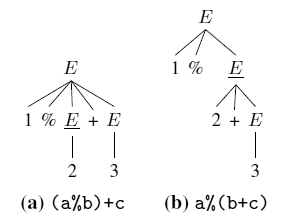
\includegraphics[scale=0.67]{Figure14.png}
\caption{Drzewa parsowania dla a\%b+c i $E\rightarrow(\%E|+E)^* $}
%i $$}
\end{figure}

Aby wybrać właściwą interpretację , generowany parser
musi porównać priorytet poprzedniego operatora do priorytetu bieżącego operatora
w $(\% E | + E)^*$ w "pętli." Na Rysunku 14, underscore{E} jest krytyczna ekspansją E.
Musi jedynie dopasować id i od
razu powrócić, pozwalając wołanemu E dopasować + do formy drzewa parsowania (a) lub odwrotnie (b).
\par
Aby obsługiwać takie porównania, produkcje dostają numer priorytetu, który jest przeciwieństwem numeru 
produkcji. Priorytet i-tej produkcji jest n-i+1 dla n \textit{oryginalnych} produkcji E.
To przypisuje priorytet 3 do $E \rightarrow E \%E$, priorytet 2 do
$E \rightarrow E + E$ i priortyet 1 do $E \rightarrow id$.
\par
Następnie każde zagnieżdżone wywołanie E potrzebuje informacji 
o priorytecie operatora z wołanego E. Najprostszym mechanizmem
jest włożenie parametru priorytetu pr do E:
\textit{Rozwinięcie E[pr] może dopasować jedynie te podwyrażenia
których priorytet odpowiada albo przekracza pr.}
\par
By zmusić do tego, procedura eliminacji lewostronnej rekurencji 
wstawia predykaty do pętli (\% E | + E)*. Tutaj jest transformowana
jednoznaczna i nie lewostronnie rekurencyjna reguła:
\par
$E[pr] \rightarrow \textbf{id} (\{ 3 \geq pr\}? \%E[4]| \{ 2 \geq pr\}?+E[3])^*$
\par
Odniesienia do E wszędzie w gramatyce stają się E[0]: czyli $S\rightarrow E$ staje się $S\rightarrow E[0]$.
Wejście a\%b+c daje drzewo parsowania dla E[0] pokazane na (a) obrazka 15.
\begin{figure}[h]
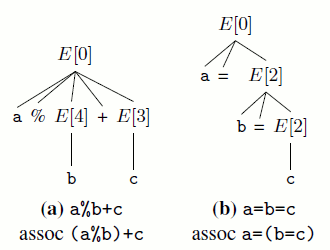
\includegraphics[scale=0.67]{Figure15.png}
\caption{Drzewa Rozwinięcia Nieterminali dla nieterminalu
$E[pr]\rightarrow id (\{3 \geq pr \}? \%E[4]|\{2 \geq pr \}? +E[3])^* $}
%i $$}
\end{figure}
\par
Produkcja “$\{ 3 \geq pr\}? \%E[4]$” jest wykonalna kiedy priorytet
operacji modulo 3, odpowiada lub przekracza parametr pr.
Pierwsze wołanie E ma pr = 0 i ponieważ $3 \geq 0$
parser rozwija “\% E[4]” w E[0].
\par
Kiedy wołamy parsowanie E[4], predykat $ {2 \geq pr}?$ nie przechodzi
ponieważ priorytet operatora + jest zbyt niski: $2 \ngeq 4$.
Konsekwentnie E[4] nie dopasowuje operatora + opóźniając
wołanie E[0].
\par
Kluczowym elementem transformacji jest wybór 
parametrów E, E[4] i E[3] w tej gramatyce. Dla operatorów lewostronnej łączności
jak \% i +, prawy operand dostaje o jeden stopień priorytetu więcej niż sam operator.
To gwarantuje że wołanie E dla prawego operandu dopasuje wyłącznie operacje wyższego priorytetu.
\par
Dla prawostronnie łącznych operacji. operand E dostaje ten sam priorytet
co bieżący operator. Tutaj jest wariacja gramatyki wyrażenia która ma prawostronny 
operator przypisania zamiast operatora dodawania:
\par
$E \rightarrow E \% E |E =^right E | \textbf{id}$
\par
gdzie notacja =^right jest skrótem dla rzeczywistej ANTLR
składni “|<assoc=right> E =^right E.” 
Interpretacja a=b=c powinna być prawostronnie łącznam a=(b=c). Aby dostać łączność,
transformowana reguła potrzebuje różnić się wyłącznie w prawym 
operandzie, E[2] kontra E[3]:
\par
$E[pr] \rightarrow \textbf{id} (\{3 \geq pr\}? \%E[4] |\{2\geq pr\}? = E[2])*$
\par
Rozwinięcie E[2] może dopasować przypisanie jak pokazano na (b) Obrazka 15, ponieważ predykat
$2 \geq 2$ jest true.
\par
Operatory unarnych prefiksów i sufiksów są natomiast traktowane jako prawe lewostronnie łączne.
Rozważmy następujące E z prefiksem negacji i sufiksem „not”.
\par
$E \rightarrow -E |E !|E \%E | \textbf{id}$
\par
Operatory prefiksu nie są lewostronnie rekurencyjne i stąd idą do
pierwszej podreguły podczas gdy lewostronnie rekurencyjne operaotry sufiksu idą do pętli predykatu 
jak operatory binarne:
\par
$E[pr] \rightarrow (id | - E[4])$
$(\{3 |wieksze_rowne pr\}? !| \{2 \geq pr\}? \%E[3])*$
\begin{figure}[h]
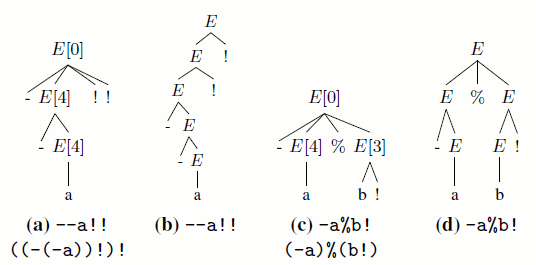
\includegraphics[scale=0.67]{Figure16.png}
\caption{Drzewa wołania nieterminali i drzewa parsowania dla prdukcji
$E\rightarrow-E|E!|E\%E|id$}
%i $$}
\end{figure}
Obrazek 16 ilustruje drzewo wołania reguł (zapis stosu wowołań) i powiązane drzewa parsowania będące
rezultatem parsera generowanego przez ANTLR. Operacje unarne w przyległych produkcjach wszystkie mają
ten sam relatywny priorytet i są dlatego “wyliczane” w podanej kolejności.
Czyli
$E \rightarrow -E | + E | id$ musi interperatować -+a jako -(+a) nie +(-a).
\par
Nonkonformistyczne leowstronne produkcje $E \rightarrow E$ lub
$E \rightarrow \epsilon $ są przepisane bez koncentrowania się na niejednoznaczności używając typowych
technik eliminacji.
\par
Ponieważ potrzeba rozwiązania niejednoznaczności z predykatami i obliczenia parametrów A

\subsection{Reguły eliminacji lewostronnej rekursji}
Aby wyeliminować bezpośrednią lewostronną rekurencję w nie terminalach
i rozwiążać niejednoznaczność ambiguities, ANTLR patrzy na cztery wzorce:
\begin{enumerate}
\item $A_i \rightarrow A\alpha_i A$ (operator binarny i ternarny)
\item $A_i \rightarrow A\alpha_i$ (operator sufiksu)
\item $A_i \rightarrow \alpha_iA$ (operator prefisku)
\item $A_i \rightarrow \alpha_i$ (pierwotny lub “inny”)
\end{enumerate}
Indeks na prodkcji A_i , chwyta numer produkcji 
w oryginalnej gramatyce kiedy potrzeba. Ukryta lub niebezpośrednia 
lewostronna rekurencja skutkuje statycznymi błędami lewostronnej rekurencji w ANTLR.
Procedura transformacji z G do G0 jest:
\begin{enumerate}
\item Pozbaw bezpośrednio lewostronnie rekurencyjnych  nieterminali odniesień
\item Zgromadź prefiks, pierwotne produkcje do nowo utworzonego A'
\item Zgromadź binarne, ternarne i sufiksowe produkcje to nowo utworzonego A''
\item Produkcje prefiksowe w A'' z semantyką sprawdzania priorytetu predykat
\{pr(i)>= pr\} gdzie pr(i) = \{n- i + 1\}
\item Przepisz odniesienia A pośród binarnych, ternarnych, i prefiksowych produkcji
jako A[nextpr(i, assoc)] gdzie
nextpr(i, assoc) = \{assoc == left ? i + 1 : i\}
\item Przepisz jakiekolwiek inne odnieisenia A w produkcji P
(włączając A0 i A00) jako A[0]
\item Przepisz oryginalną regułę A jako A[pr] $\rightarrow$ A'A''
\end{enumerate}
W praktyce ANTLR używa formy EBNF zamiast A'A''.



\end{document}
